% Copyright 2019 Clara Eleonore Pavillet

% Author: Clara Eleonore Pavillet
% Description: This is an unofficial Oxford University Beamer Template I made from scratch. Feel free to use it, modify it, share it.
% Version: 1.0

\documentclass{beamer}
% Load Packages
\usepackage[utf8]{inputenc}
\usepackage{xcolor}
\usepackage{tikz}
\usetikzlibrary{positioning,calc}
\usepackage{graphicx}
\usepackage{hyperref}
\usepackage{amsmath}
\usepackage{listings}
\usepackage{fontawesome}

% Define Commands
\newcommand*{\ClipSep}{0.06cm} %To adjust footer logo
\newcommand{\E}{\mathrm{e}\,} %\def\I{e} % used to defined e for exp(x), see later what it should be
\newcommand{\ud}{\mathrm{d}}
\lstset{numbers=left, numberstyle=\tiny, stepnumber=1,firstnumber=1,breaklines=true,
    numbersep=5pt,language=Python,
    stringstyle=\ttfamily,
    basicstyle=\footnotesize, 
    showstringspaces=false
}

\usetheme{oxonian}

\usepackage{graphicx}
\usepackage{subfigure}

\title{Driver de Dois Estágios para Acionamento	de EHC COB LEDs}
\titlegraphic{
\includegraphics[width=8cm]{Theme/Logos/logo.png}}
\author{Eric Gonçalves Pusiol}
\institute{UFJF}
\date{} %\today

\usepackage[brazil]{babel}

\begin{document}

{\setbeamertemplate{footline}{} 
\frame{\titlepage}}

\section*{Índice}\begin{frame}{Índice}\tableofcontents\end{frame}

\section{Introdução}
\begin{frame}[plain]
	\vfill
	\centering
	\begin{beamercolorbox}[sep=8pt,center,shadow=true,rounded=true]{title}
		\usebeamerfont{title}\insertsectionhead\par%
		\color{oxfordblue}\noindent\rule{10cm}{1pt}
	\end{beamercolorbox}
	\vfill
\end{frame}
%----------------------------------------------------------
\begin{frame}{Introdução}
	No tópico de iluminação moderna, temos os EHC COB LEDs. Suas características são:

	\begin{enumerate}
		\item Alta potência e alto fluxo
		\item Compactos
		\item Elevada dissipação de calor
		\item Baixa tensão e alta corrente
	\end{enumerate}
\end{frame}
%----------------------------------------------------------

\subsection{EHC COB LEDs}
\begin{frame}{EHC COB LEDs}
		
\begin{figure}[htb]
	\centering
	\mbox{
		\subfigure[Ilustração de um COB LED]{
			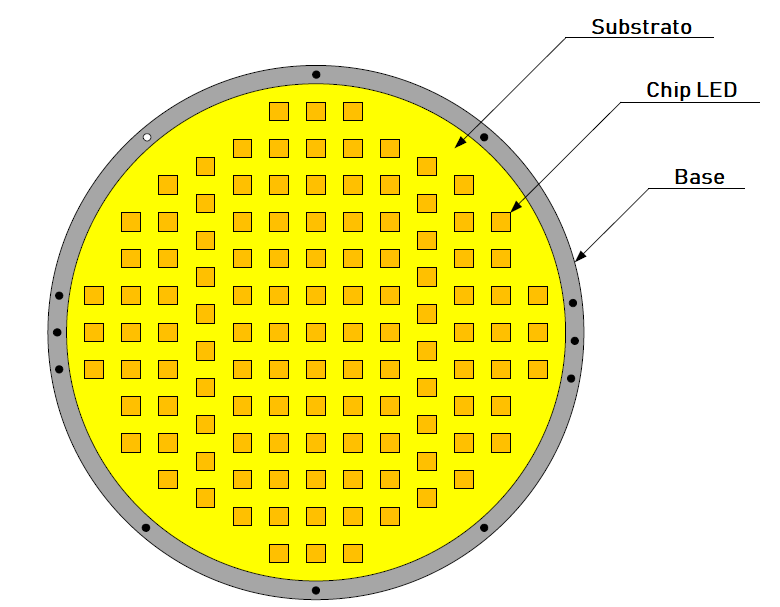
\includegraphics[width=4cm]{../../FIGURAS/cob.png}}\qquad
		\subfigure[Apollo 600 com dissipador]{
			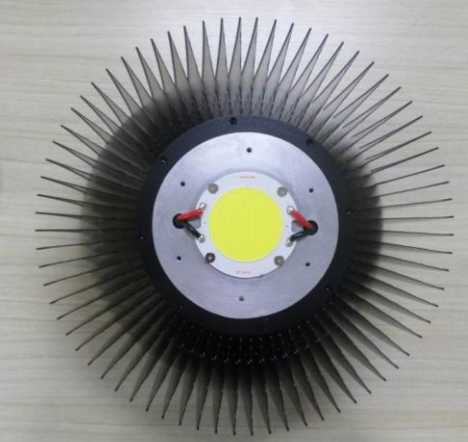
\includegraphics[width=4cm]{i/apolo.png}}
	}
	\caption{COB LEDs}
\end{figure}

\end{frame}
%----------------------------------------------------------


\subsection{Especificações}
\begin{frame}{Introdução}
\begin{table}[!h]
	\centering
	\caption[Valores máximos dos parâmetros elétricos, térmicos e fotométricos do EHC COB LED Apollo 600.]{%
		\parbox[t]{10cm}{Valores máximos dos parâmetros elétricos, térmicos e fotométricos do EHC COB LED Apollo 600.}}
	\begin{tabular}{|l|l|}
		\hline
		Dissipação máxima de potência     & 608,4 W                                     \\ \hline
		Máxima corrente CC de operação    & 12 A                                        \\ \hline
		Máxima temperatura de junção      & 140$^\circ$ C \\ \hline
		Temperatura de cor correlata      & 5000 K                                      \\ \hline
		Fluxo luminoso na corrente máxima & 60840 lm                                    \\ \hline
	\end{tabular}
	\label{apollo-spec}
\end{table}
\end{frame}

%----------------------------------------------------------
\section{Arquitetura em Dois Estágios}
\begin{frame}[plain]
	\vfill
	\centering
	\begin{beamercolorbox}[sep=8pt,center,shadow=true,rounded=true]{title}
		\usebeamerfont{title}\insertsectionhead\par%
		\color{oxfordblue}\noindent\rule{10cm}{1pt}
	\end{beamercolorbox}
	\vfill
\end{frame}
%----------------------------------------------------------
\begin{frame}{Arquitetura em Dois Estágios}

\begin{figure}[htb]
	\centering
		\includegraphics[width=8cm]{../../ESQUEMAS/twostage.png}
		\caption{Conversor em dois estágios}
\end{figure}
	
\end{frame}
%----------------------------------------------------------
\begin{frame}{Arquitetura em Dois Estágios}
	
\begin{figure}[htb]
	\centering
	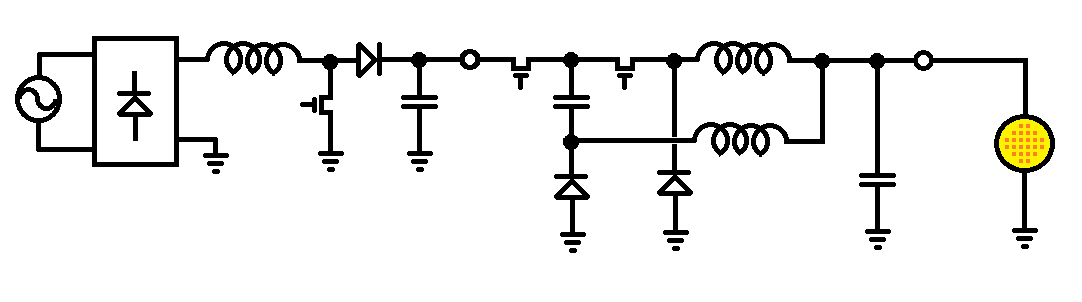
\includegraphics[width=12cm]{../../ESQUEMAS/BOOST_EDSCIBUCK.png}
	\caption{Conversor em dois estágios}
\end{figure}
	
\end{frame}
%----------------------------------------------------------
\subsection{Primeiro Estágio}
\begin{frame}{Primeiro Estágio}
	
	\begin{figure}[htb]
		\centering
		\includegraphics[width=8cm]{../../ESQUEMAS/boost.png}
		\caption{\textit{Conversor \textit{Buck} off-line}}
	\end{figure}
	
\end{frame}
%----------------------------------------------------------
\begin{frame}{Controle CMC}
	
	\begin{figure}[htb]
		\centering
		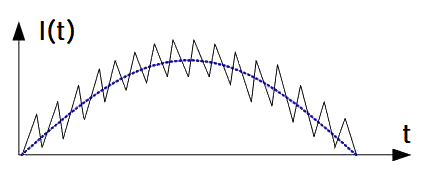
\includegraphics[width=8cm]{../../RABISCOS/cmc_wav}
		\caption{Corrente no indutor em um conversor \textit{boost} PFC CCM}
	\end{figure}
	
\end{frame}
%----------------------------------------------------------
\begin{frame}{Controle CMC}
	
	\begin{figure}[htb]
		\centering
		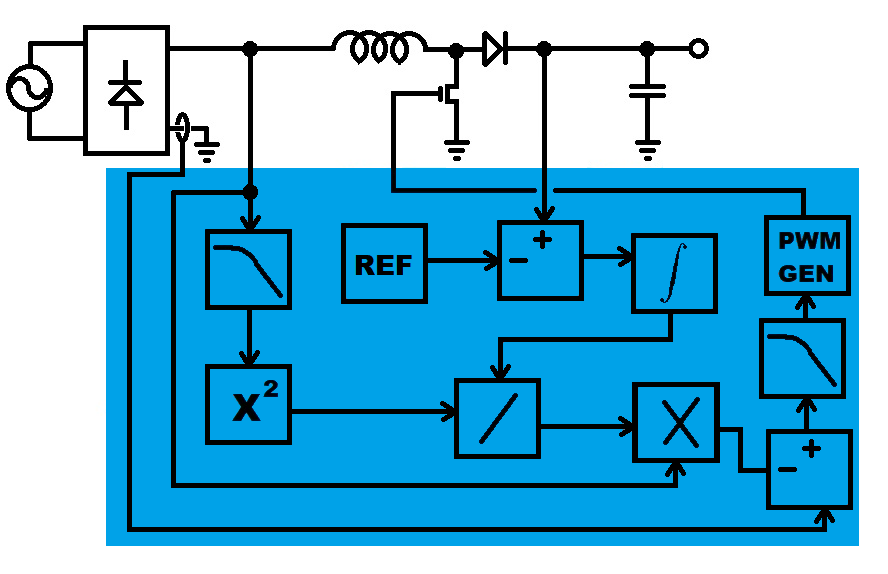
\includegraphics[width=8cm]{../../ESQUEMAS/PFC_CTRL.png}
		\caption{Esquema de controle CMC}
	\end{figure}
	
\end{frame}
%----------------------------------------------------------
\begin{frame}{Controle CMC}
	
	\begin{figure}[htb]
		\centering
		\mbox{
			\subfigure[Filtro de compensação feed-foward]{
				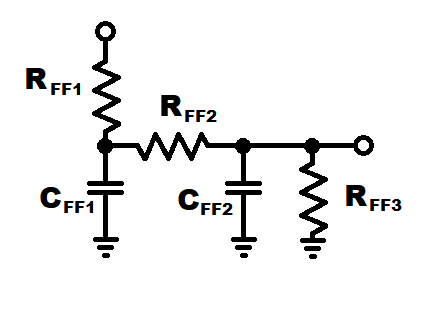
\includegraphics[height=2cm]{../../ESQUEMAS/vff}}\qquad
			\subfigure[Integrador da tensão de barramento]{
				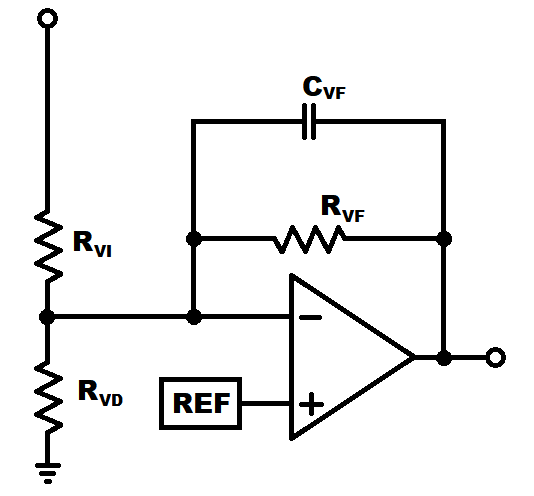
\includegraphics[height=2cm]{../../ESQUEMAS/vfo}}
		}
	\end{figure}
	
	\begin{figure}[htb]
		\centering
		\mbox{
			\subfigure[Compensador de corrente]{
				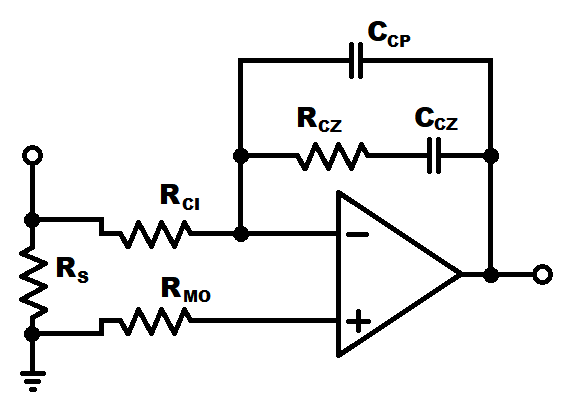
\includegraphics[height=2cm]{../../ESQUEMAS/vci}}
		}
	\end{figure}
	
\end{frame}
%----------------------------------------------------------
\begin{frame}{UC3854}
	
	\begin{figure}[htb]
		\centering
		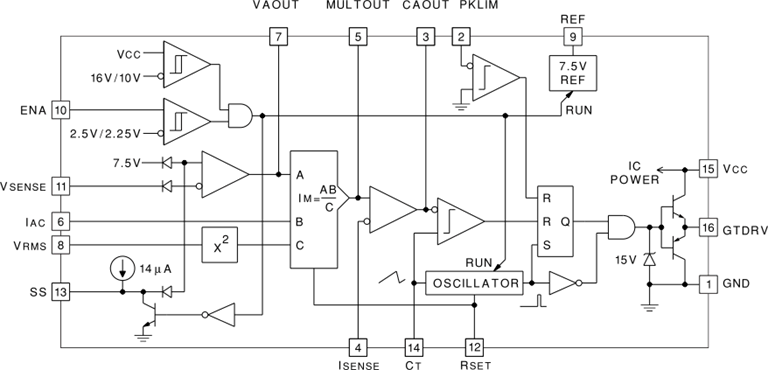
\includegraphics[width=8cm]{../../RABISCOS/fbd_slus336a.png}
		\caption{Circuito integrado que implementa CMC}
	\end{figure}
	
\end{frame}
%----------------------------------------------------------
\begin{frame}{Simulação}
	
	\begin{figure}[htb]
		\centering
		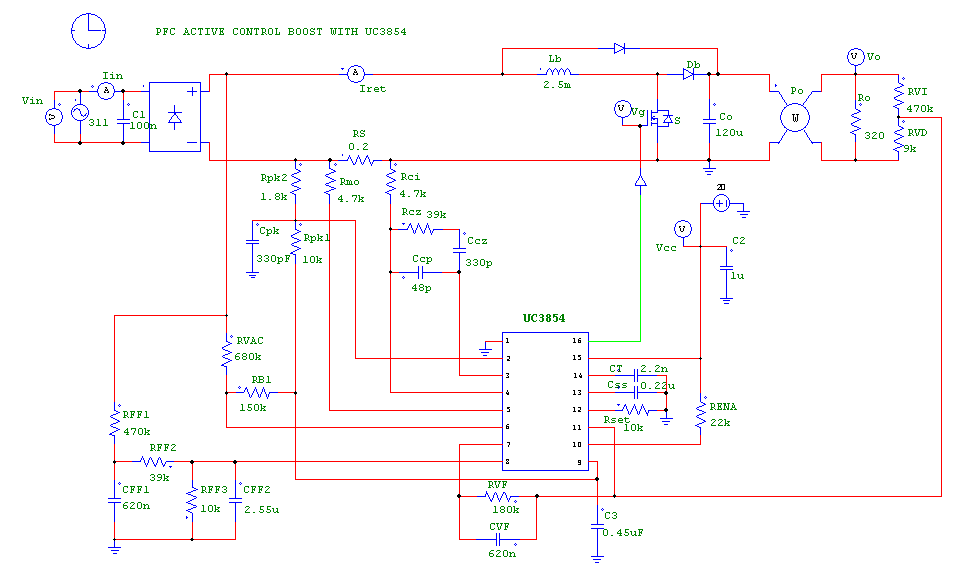
\includegraphics[width=8cm]{../../ESQUEMAS/PFC_BOOST.png}
		\caption{Circuito a ser implementado}
	\end{figure}
	
\end{frame}
%----------------------------------------------------------
\begin{frame}{Simulação}
	
\begin{figure}[htb]
	\centering
	\mbox{
		\subfigure[Saída nominal do conversor]{
			\includegraphics[height=4cm]{../../GRAFICOS/PFC_OUTPUT.png}}\qquad
		\subfigure[Conversor sujeito a distúrbio]{
			\includegraphics[height=4cm]{../../GRAFICOS/PFC_PERTUB.png}}
	}
	\caption{Formas de onda de simulação}
\end{figure}
	
\end{frame}
%----------------------------------------------------------
\subsection{Segundo Estágio}
\begin{frame}{Segundo Estágio}
	No segundo estágio será adotada uma topologia de ordem 4.
	
	\begin{figure}[htb]
		\centering
		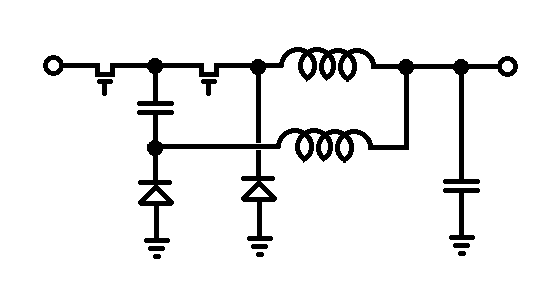
\includegraphics[width=8cm]{../../ESQUEMAS/_EDSCIBUCK_PNT.png}
		\caption{\textit{Extended Duty Cycle Series Capacitor Interleaved Buck Converter}}
	\end{figure}
	
\end{frame}
%----------------------------------------------------------
\begin{frame}{Segundo Estágio}
	\begin{figure}[htb]
		\centering
		\mbox{
			\subfigure[Etapas de operação]{
				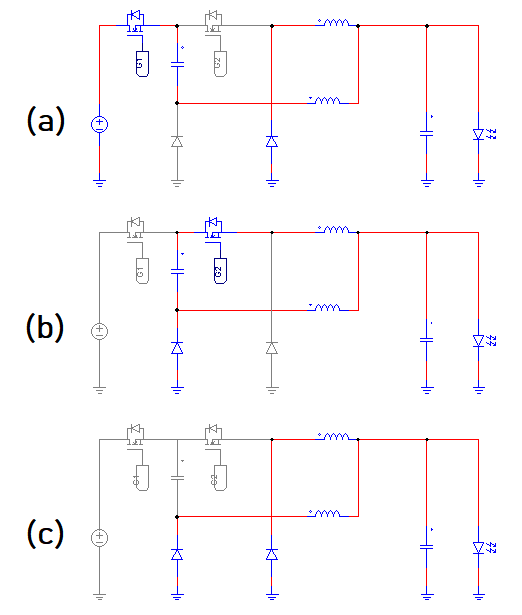
\includegraphics[height=6cm]{../../ESQUEMAS/split.png}}\qquad
			\subfigure[Formas de onda]{
				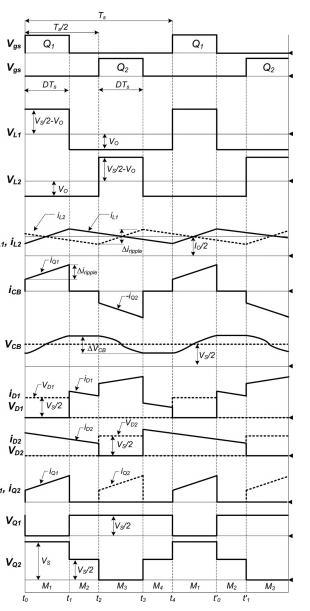
\includegraphics[height=6cm]{I/opmod.png}}
		}
		\caption{Funcionamento do Segundo estágio}
	\end{figure}
\end{frame}
%----------------------------------------------------------
%\begin{frame}{Controle Digital}
%	\begin{figure}[htb]
%		\centering
%		\mbox{
%			\subfigure[Etapas de operação]{
%				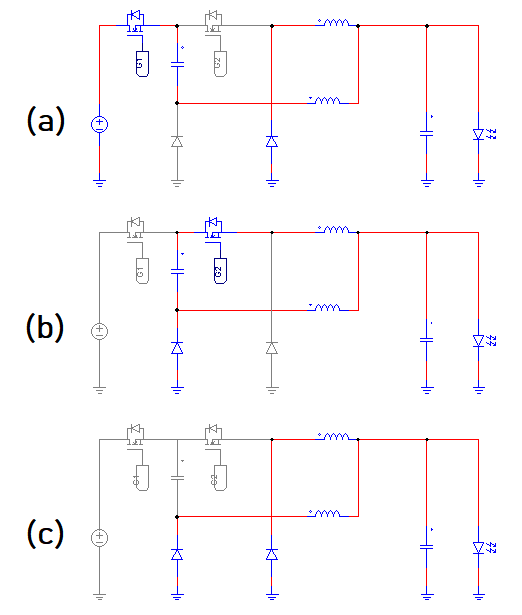
\includegraphics[height=6cm]{../../ESQUEMAS/split.png}}\qquad
%			\subfigure[Formas de onda]{
%				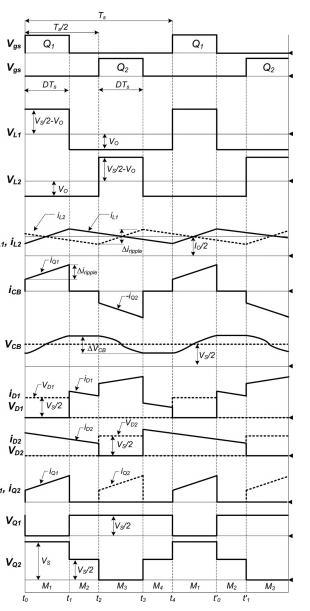
\includegraphics[height=6cm]{I/opmod.png}}
%		}
%		\caption{Funcionamento do Segundo estágio}
%	\end{figure}
%\end{frame}
%----------------------------------------------------------
\begin{frame}{Simulação}
	
	\begin{figure}[htb]
		\centering
		\includegraphics[width=8cm]{../../ESQUEMAS/ctrl_egibc_2.png}
		\caption{\textit{Extended Duty Cycle Series Capacitor Interleaved Buck Converter}}
	\end{figure}
	
\end{frame}
%----------------------------------------------------------
\begin{frame}{Simulação}
	\begin{figure}[htb]
		\centering
		\mbox{
			\subfigure[Tensões nas chaves e nos diodos e correntes nos indutores.]{
				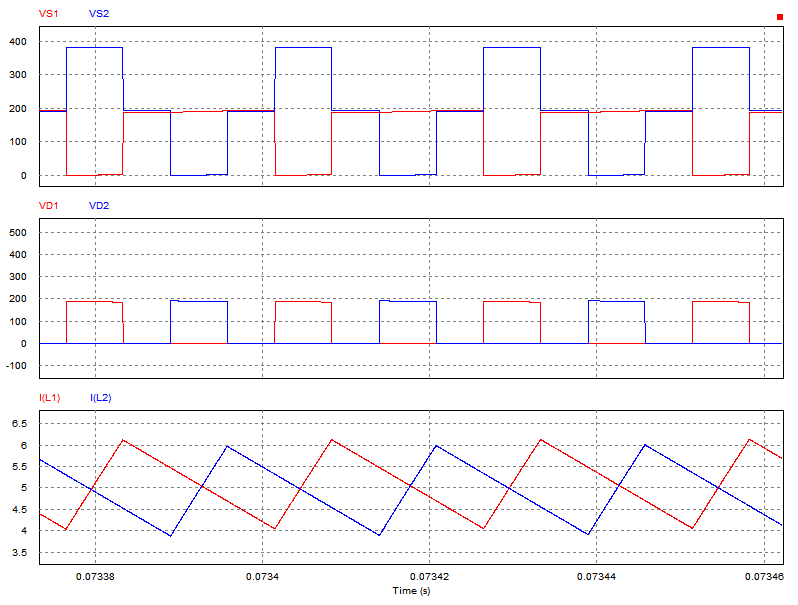
\includegraphics[height=4cm]{../../GRAFICOS/stage2_hf.png}}\qquad
			\subfigure[Saída do conversor sujeito a distúrbio]{
				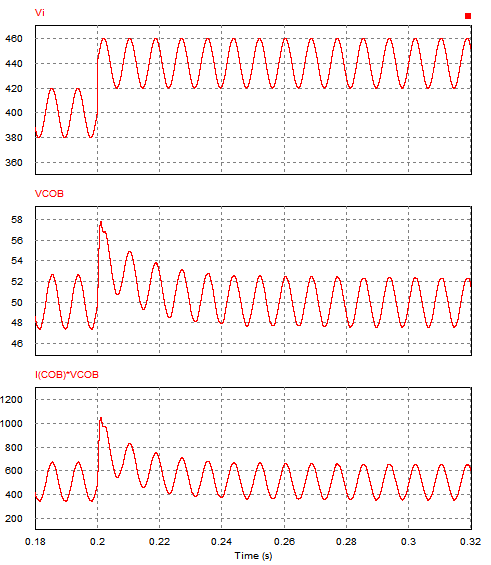
\includegraphics[height=4cm]{../../GRAFICOS/pc_disturb.png}}
		}
		\caption{Formas de onda de simulação}
	\end{figure}
\end{frame}
%----------------------------------------------------------
\section{Implementação do protótipo}
\begin{frame}[plain]
	\vfill
	\centering
	\begin{beamercolorbox}[sep=8pt,center,shadow=true,rounded=true]{title}
		\usebeamerfont{title}\insertsectionhead\par%
		\color{oxfordblue}\noindent\rule{10cm}{1pt}
	\end{beamercolorbox}
	\vfill
\end{frame}
%----------------------------------------------------------
\begin{frame}{Implementação do primeiro estágio}
\begin{table}[!h]
	\centering
	\caption[Indutor, capacitor e modelos dos semicondutores utilizados no protótipo do conversor boost PFC.]{
		\parbox[t]{10cm}{Indutor, capacitor e modelos dos semicondutores utilizados no protótipo do conversor boost PFC.}}
	\begin{tabular}{|l|l|}
		\hline
		Indutor                 & 2,7 mH    \\ \hline
		Capacitor de barramento & 160 $\mu F$    \\ \hline
		Ponte retificadora      & KBU8K     \\ \hline
		MOSFET                  & IPW60R190 \\ \hline
		Diodo                   & MUR 860   \\ \hline
		CI de controle          & UC3854   \\ \hline
	\end{tabular}
	\label{pfc-matlist}
\end{table}
\end{frame}
%----------------------------------------------------------
\subsection{Implementação do primeiro estágio}
\begin{frame}{Implementação do primeiro estágio}
	\begin{figure}[htb]
		\centering
		\mbox{
			\subfigure[Setup de teste.]{
				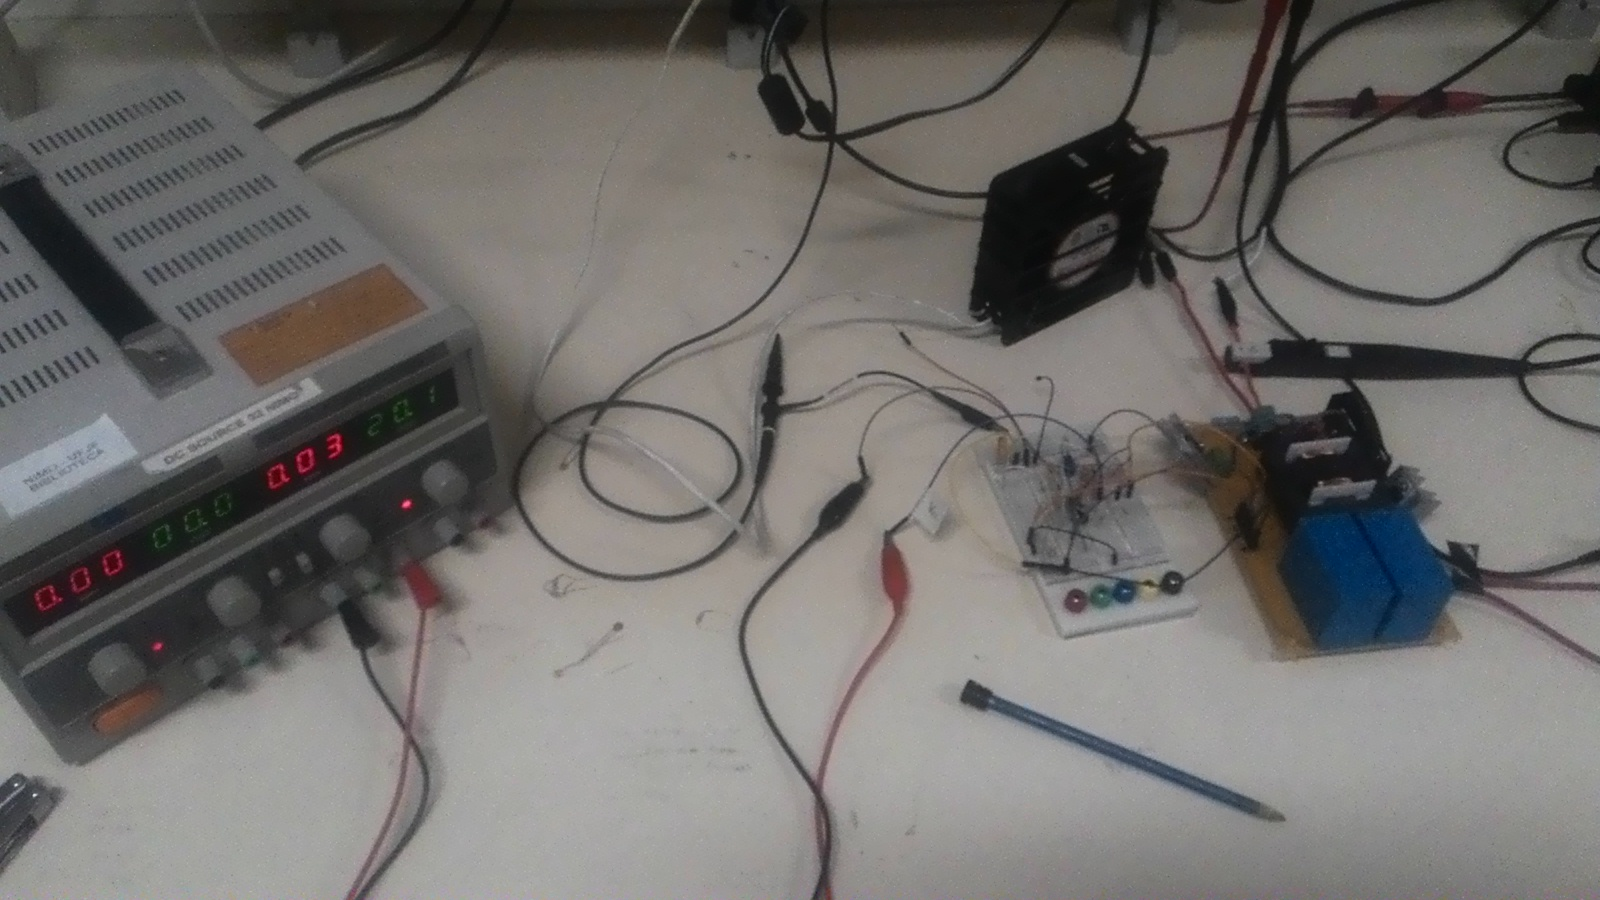
\includegraphics[height=2cm]{../../FOTOGRAFIAS/P_20180826_175623.jpg}}\qquad
			\subfigure[Placa de potência.]{
				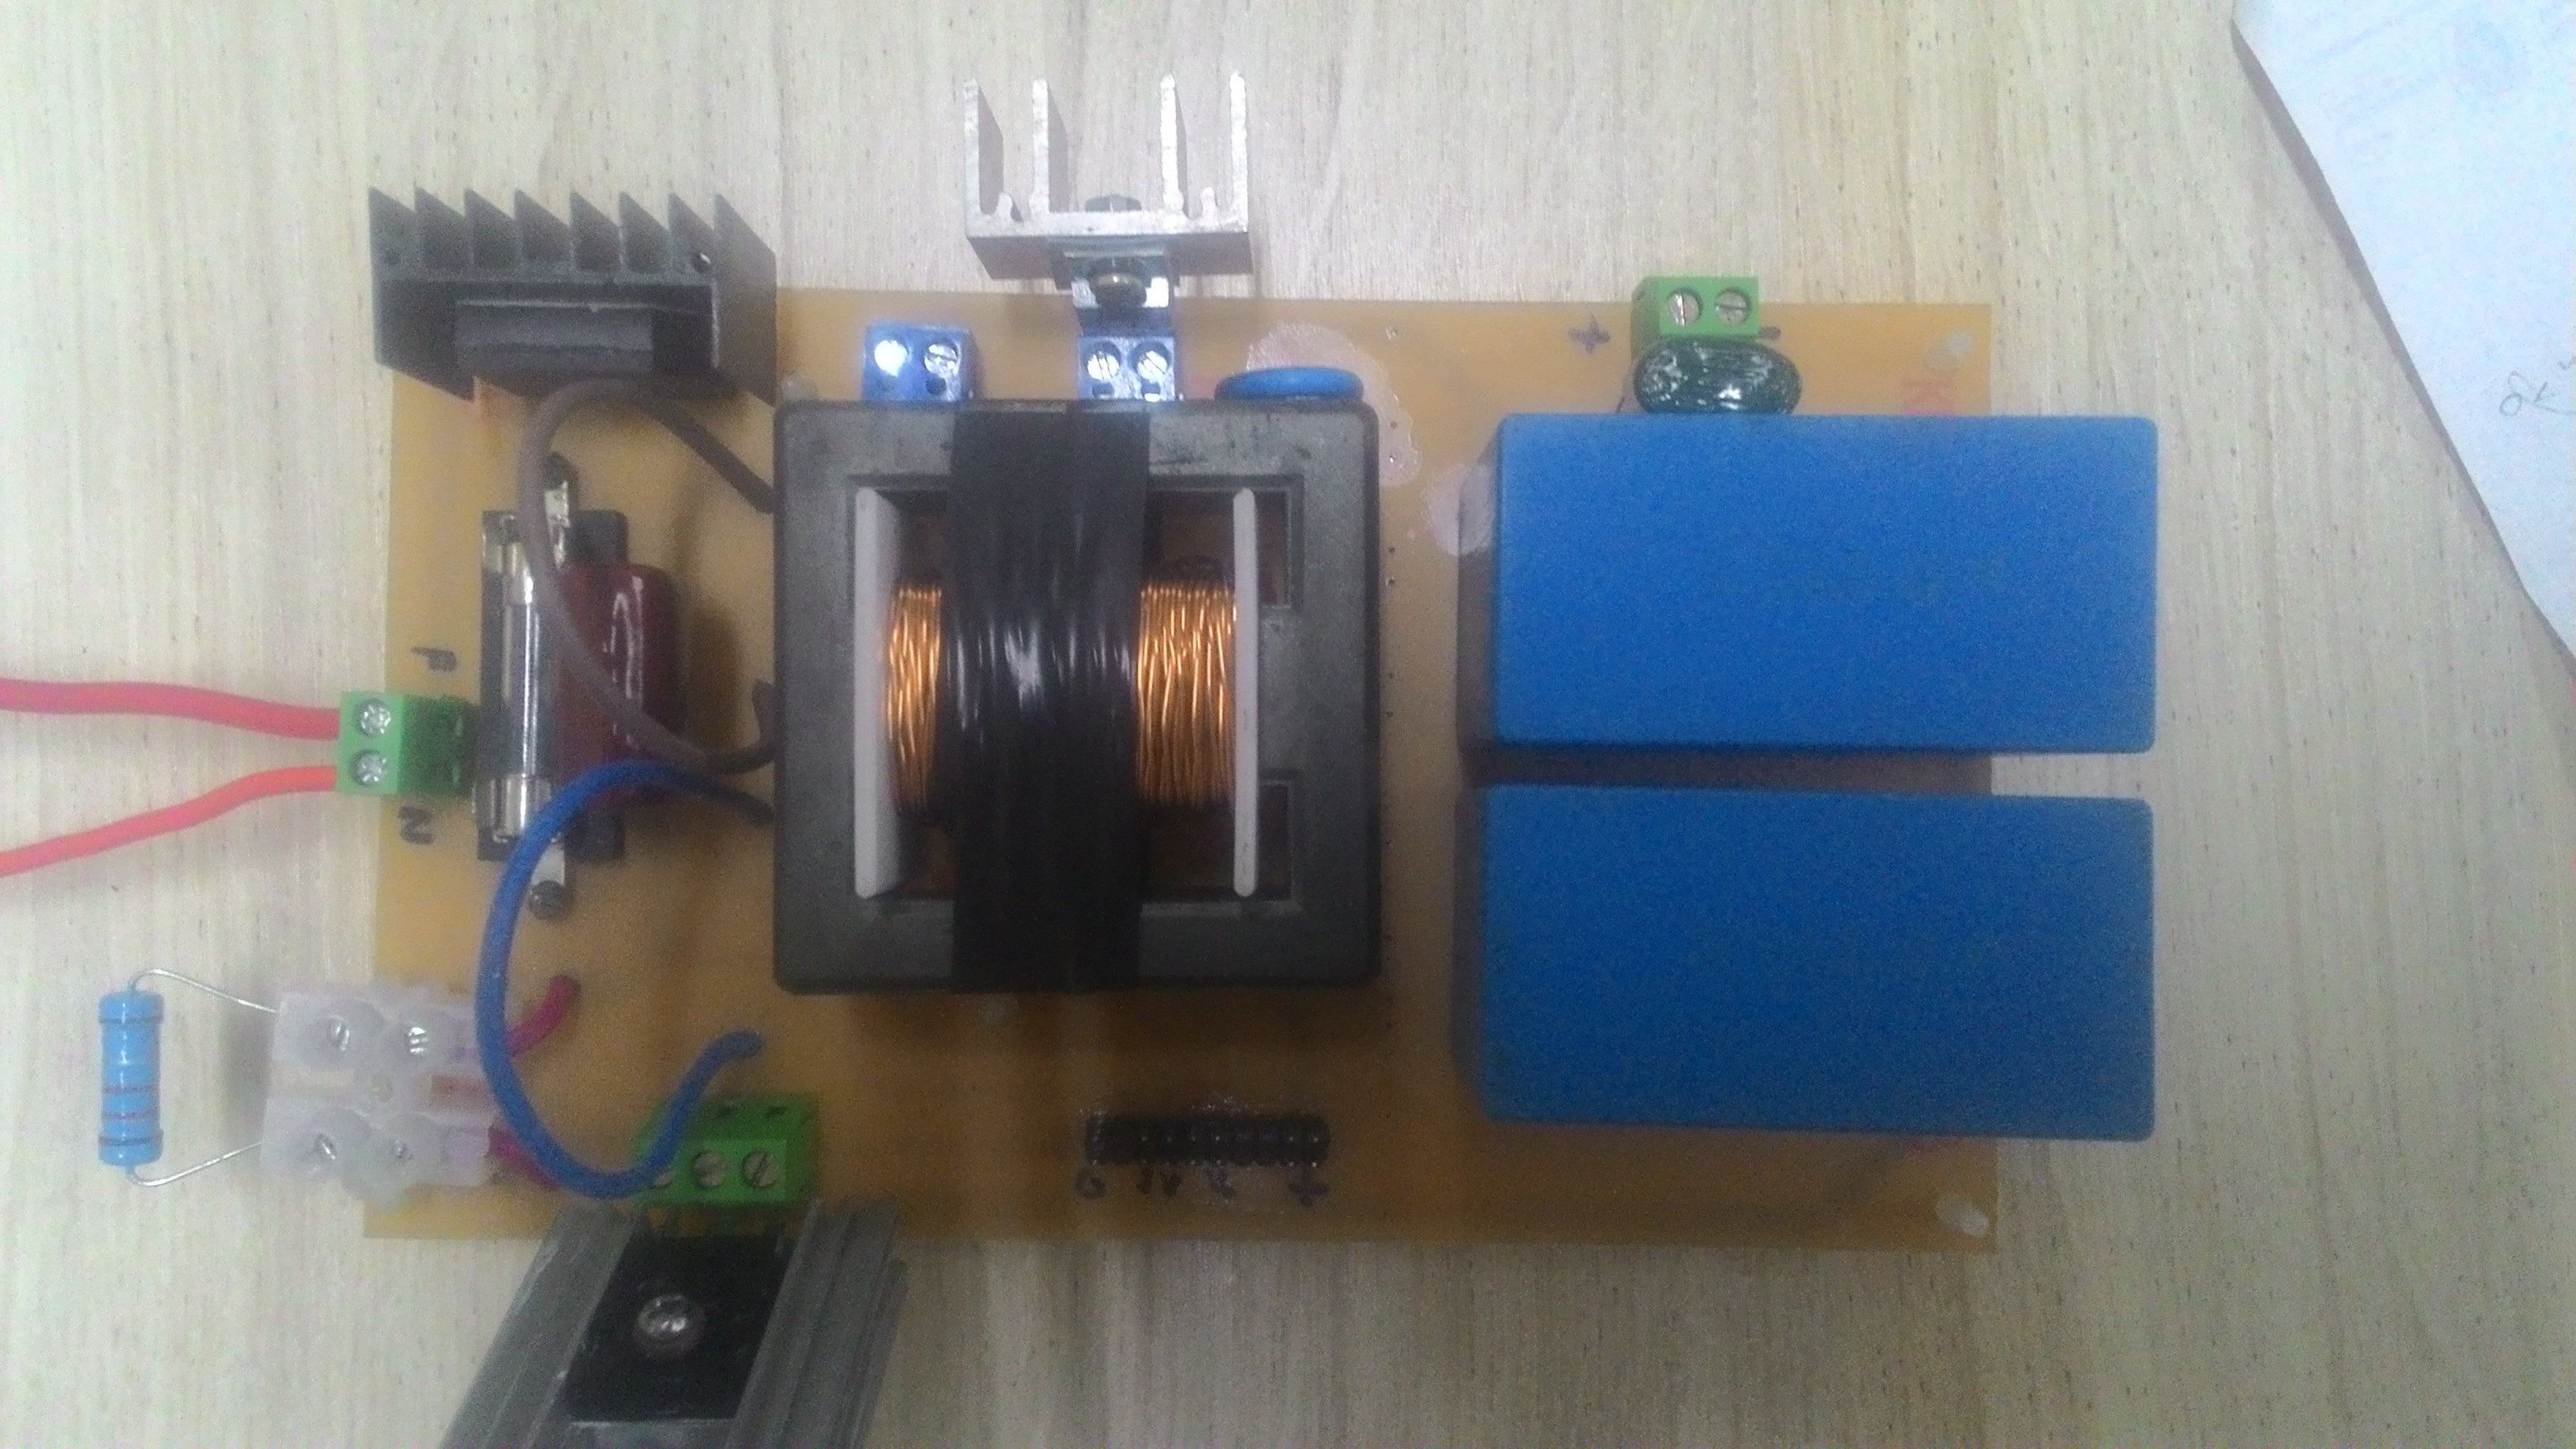
\includegraphics[height=2cm]{../../FOTOGRAFIAS/P_20180910_174425.jpg}}
		}
		\mbox{
		\subfigure[Placa de controle.]{
			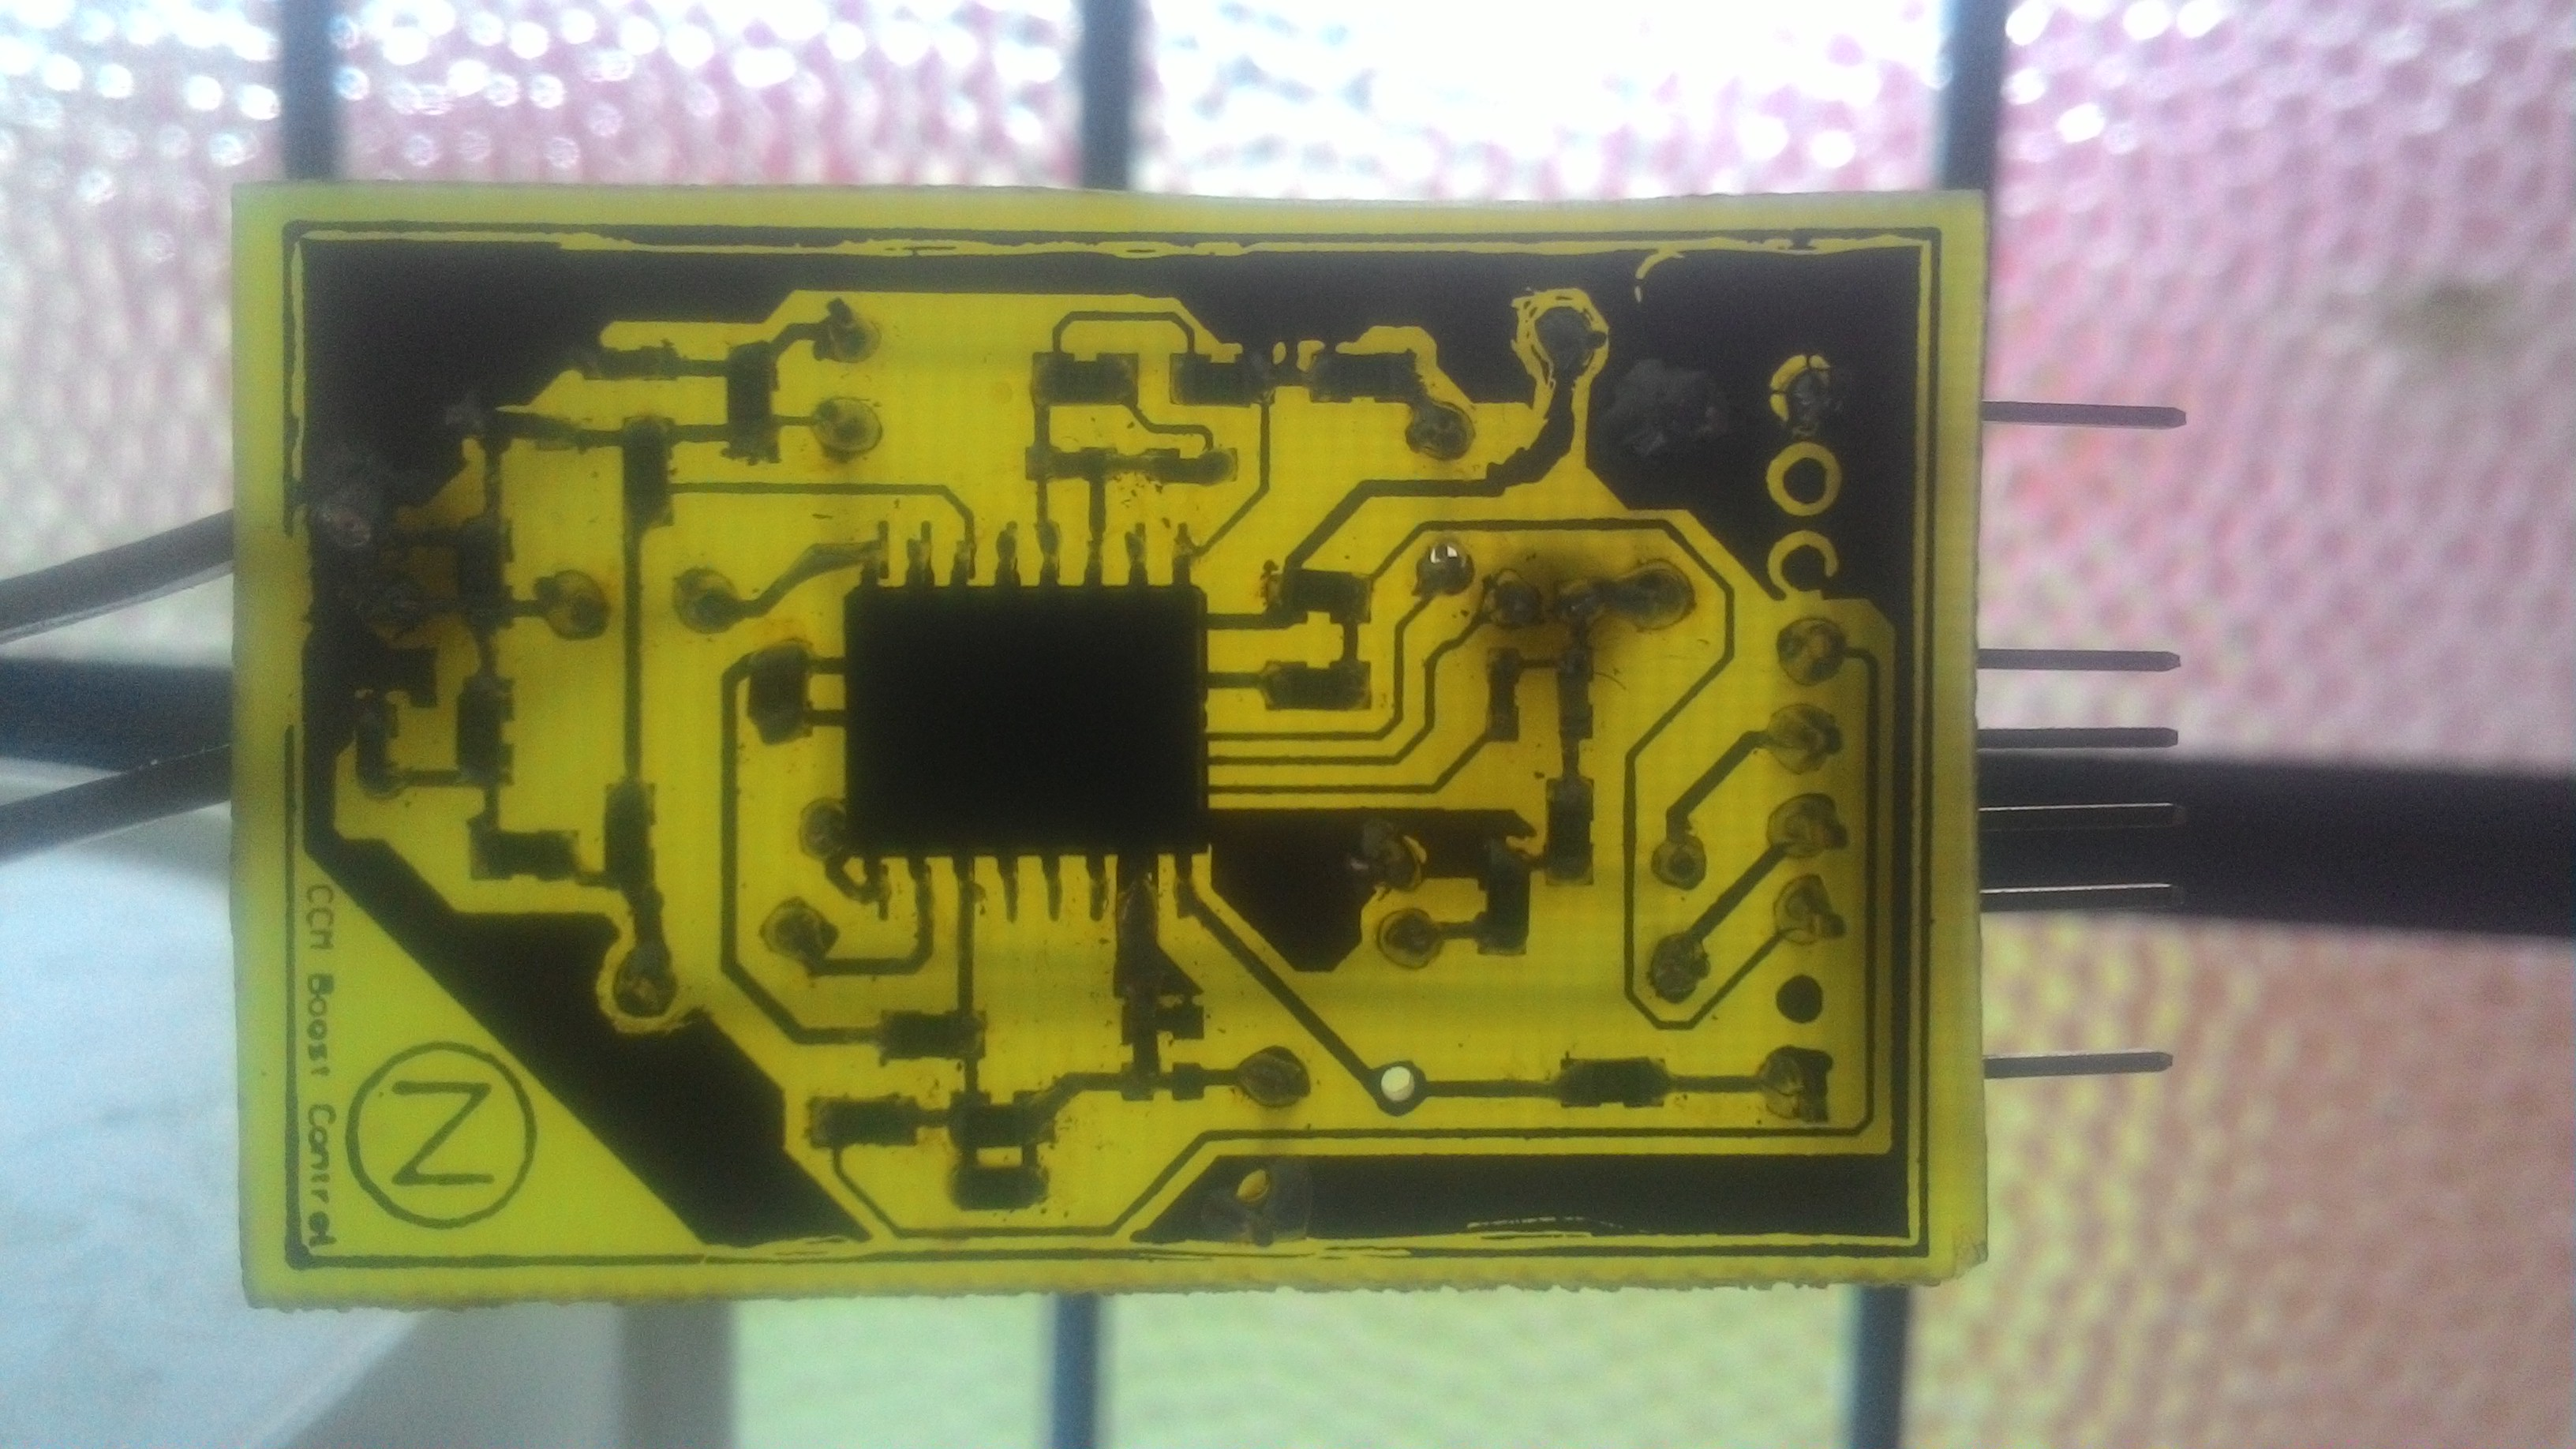
\includegraphics[height=2cm]{../../FOTOGRAFIAS/P_20180910_103427.jpg}}\qquad
		\subfigure[Denis ligando a tomada.]{
			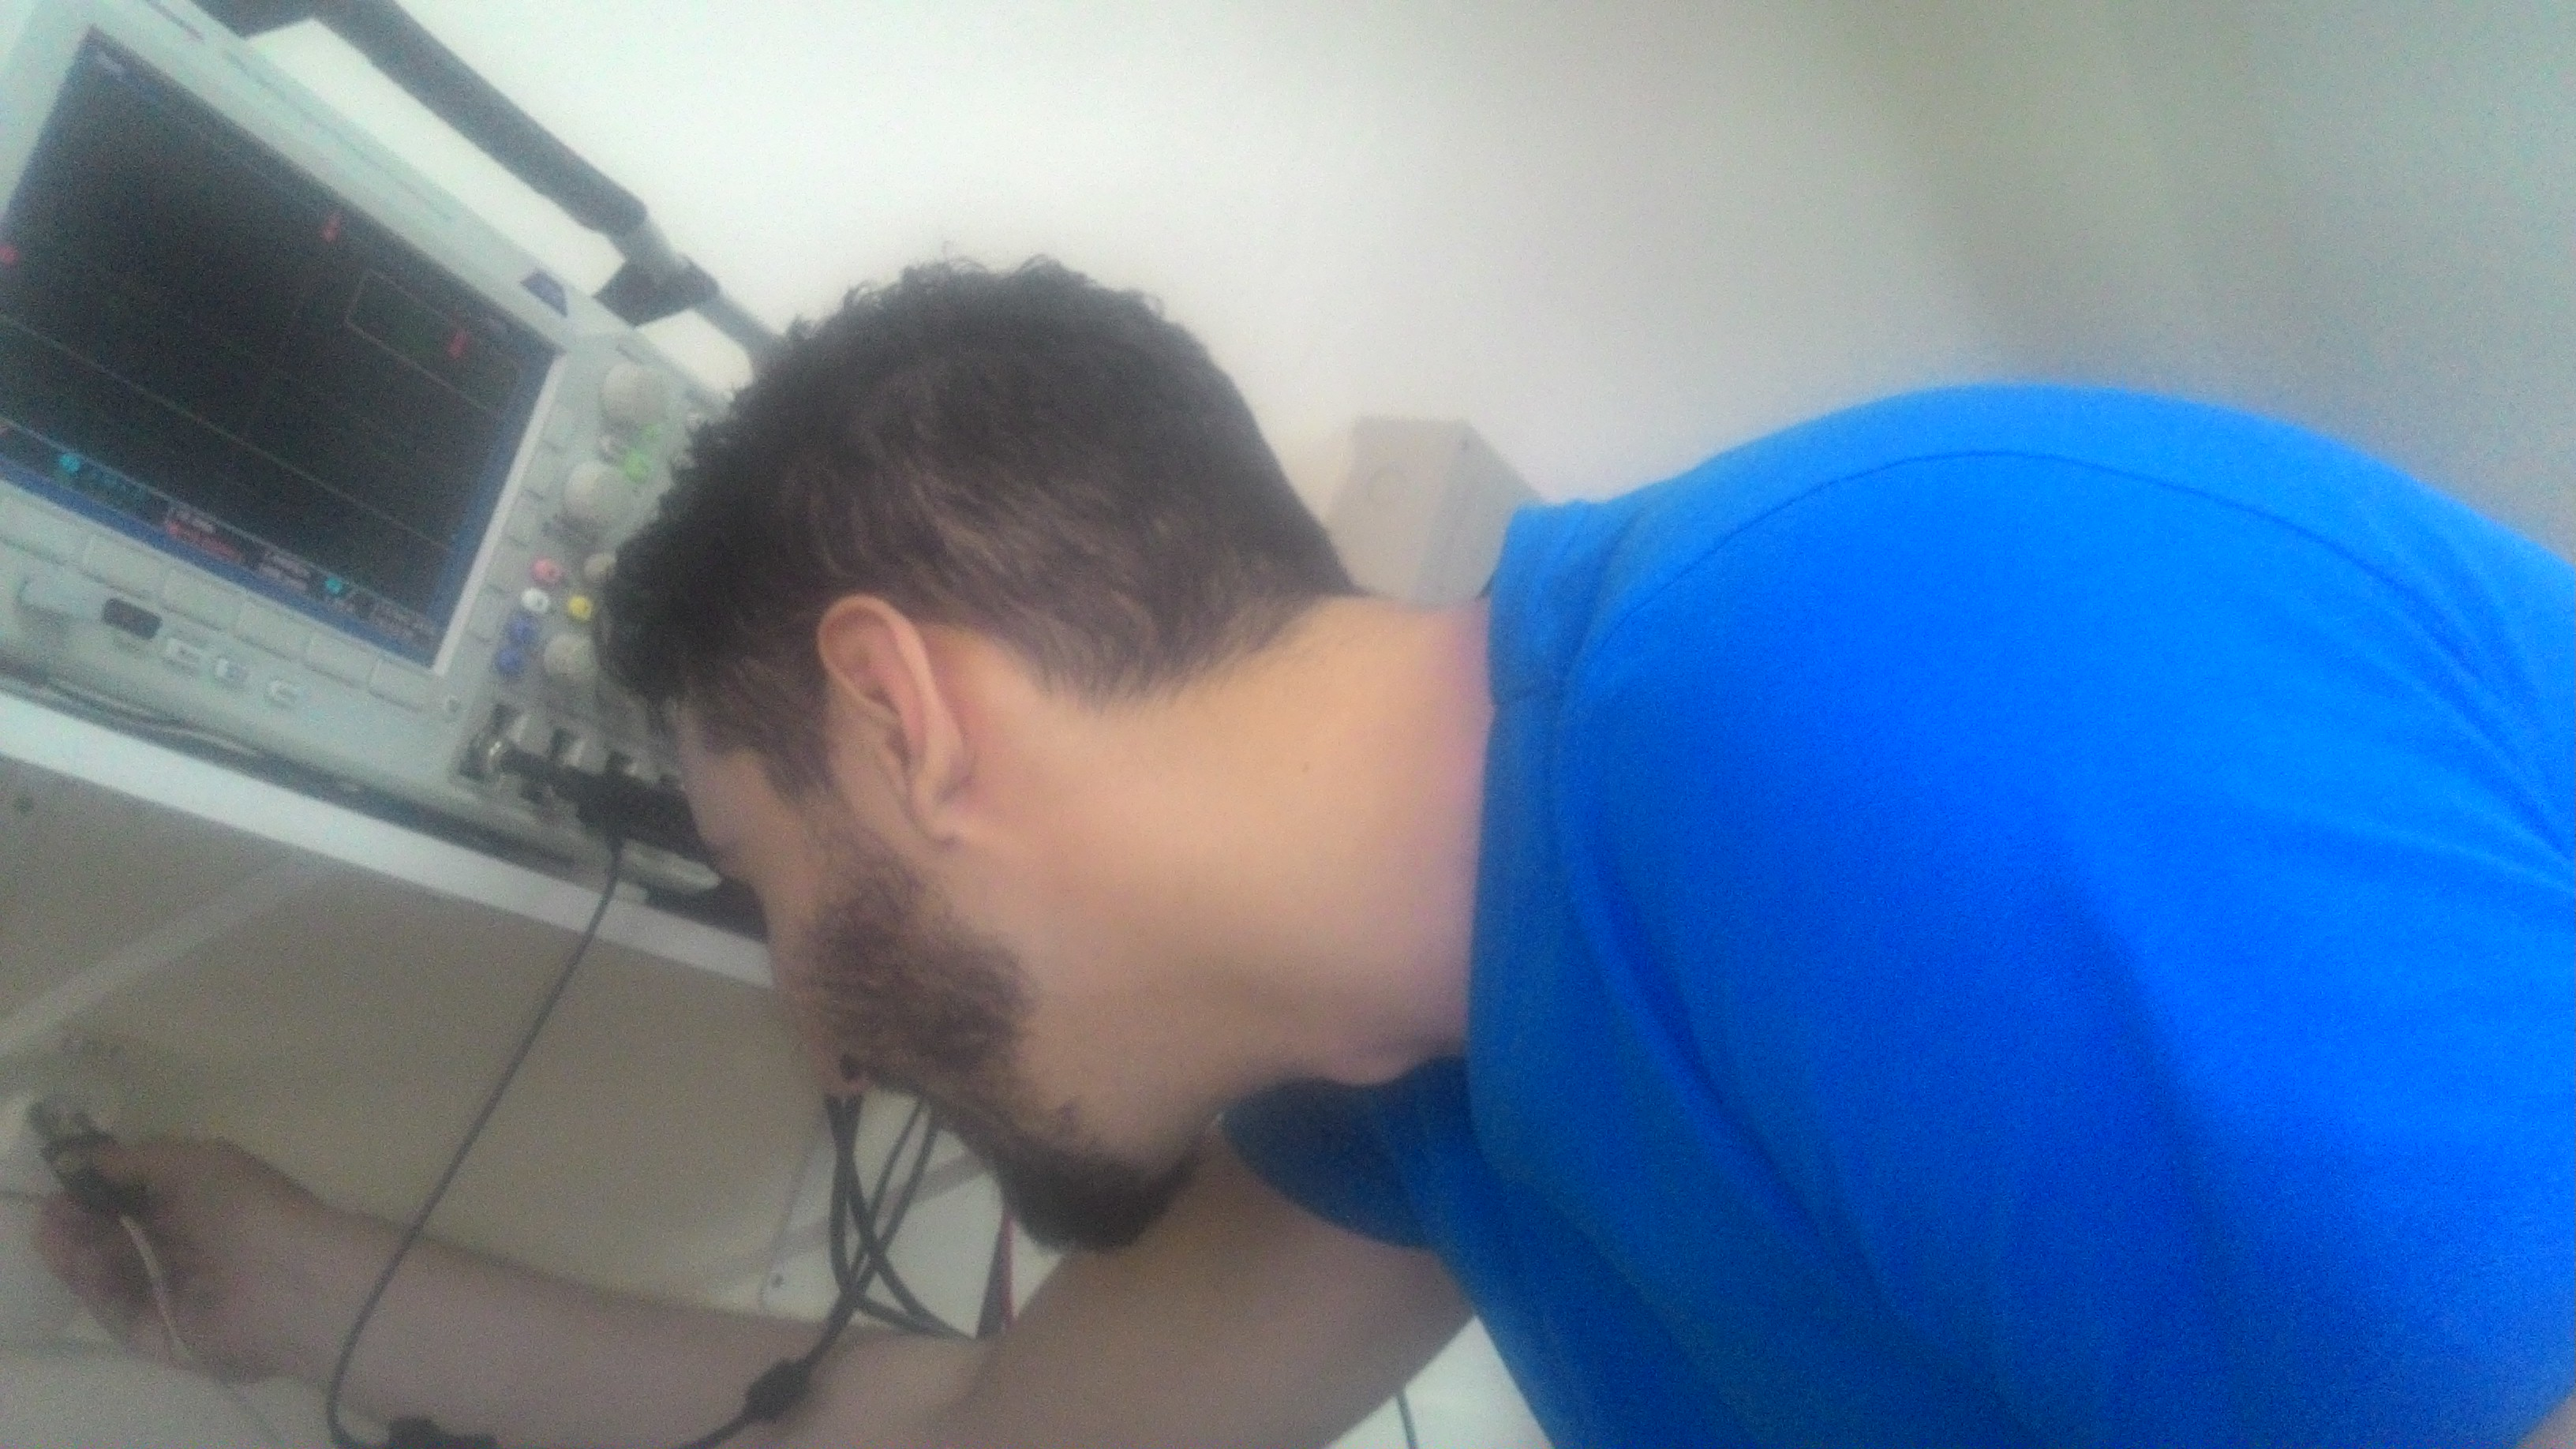
\includegraphics[height=2cm]{../../FOTOGRAFIAS/P_20181113_175207.jpg}}
	}
	\end{figure}
\end{frame}
%----------------------------------------------------------
\begin{frame}{Implementação do segundo estágio}
	\begin{table}[]
		\centering
		\caption[Indutores, capacitores e modelos dos semicondutores utilizados no protótipo do conversor EDSCIBC PC.]{
			\parbox[t]{10cm}{Indutores, capacitores e modelos dos semicondutores utilizados no protótipo do conversor EDSCIBC PC.}}
		\begin{tabular}{|l|l|}
			\hline
			Indutores                      & 500 $\mu H$ \\ \hline
			Capacitor série de acoplamento & 12 $\mu F$   \\ \hline
			Capacitor de saída             & 40 $\mu F$    \\ \hline
			MOSFETs S1 e S2                & IRFP460    \\ \hline
			Diodos D1 e D2                 & MUR 8100   \\ \hline
		\end{tabular}
		\label{pc-matlist}
	\end{table}
\end{frame}
%----------------------------------------------------------
\subsection{Implementação do segundo estágio}
\begin{frame}{Implementação do segundo estágio}
	\begin{figure}[htb]
		\centering
		\mbox{
			\subfigure[Setup de teste.]{
				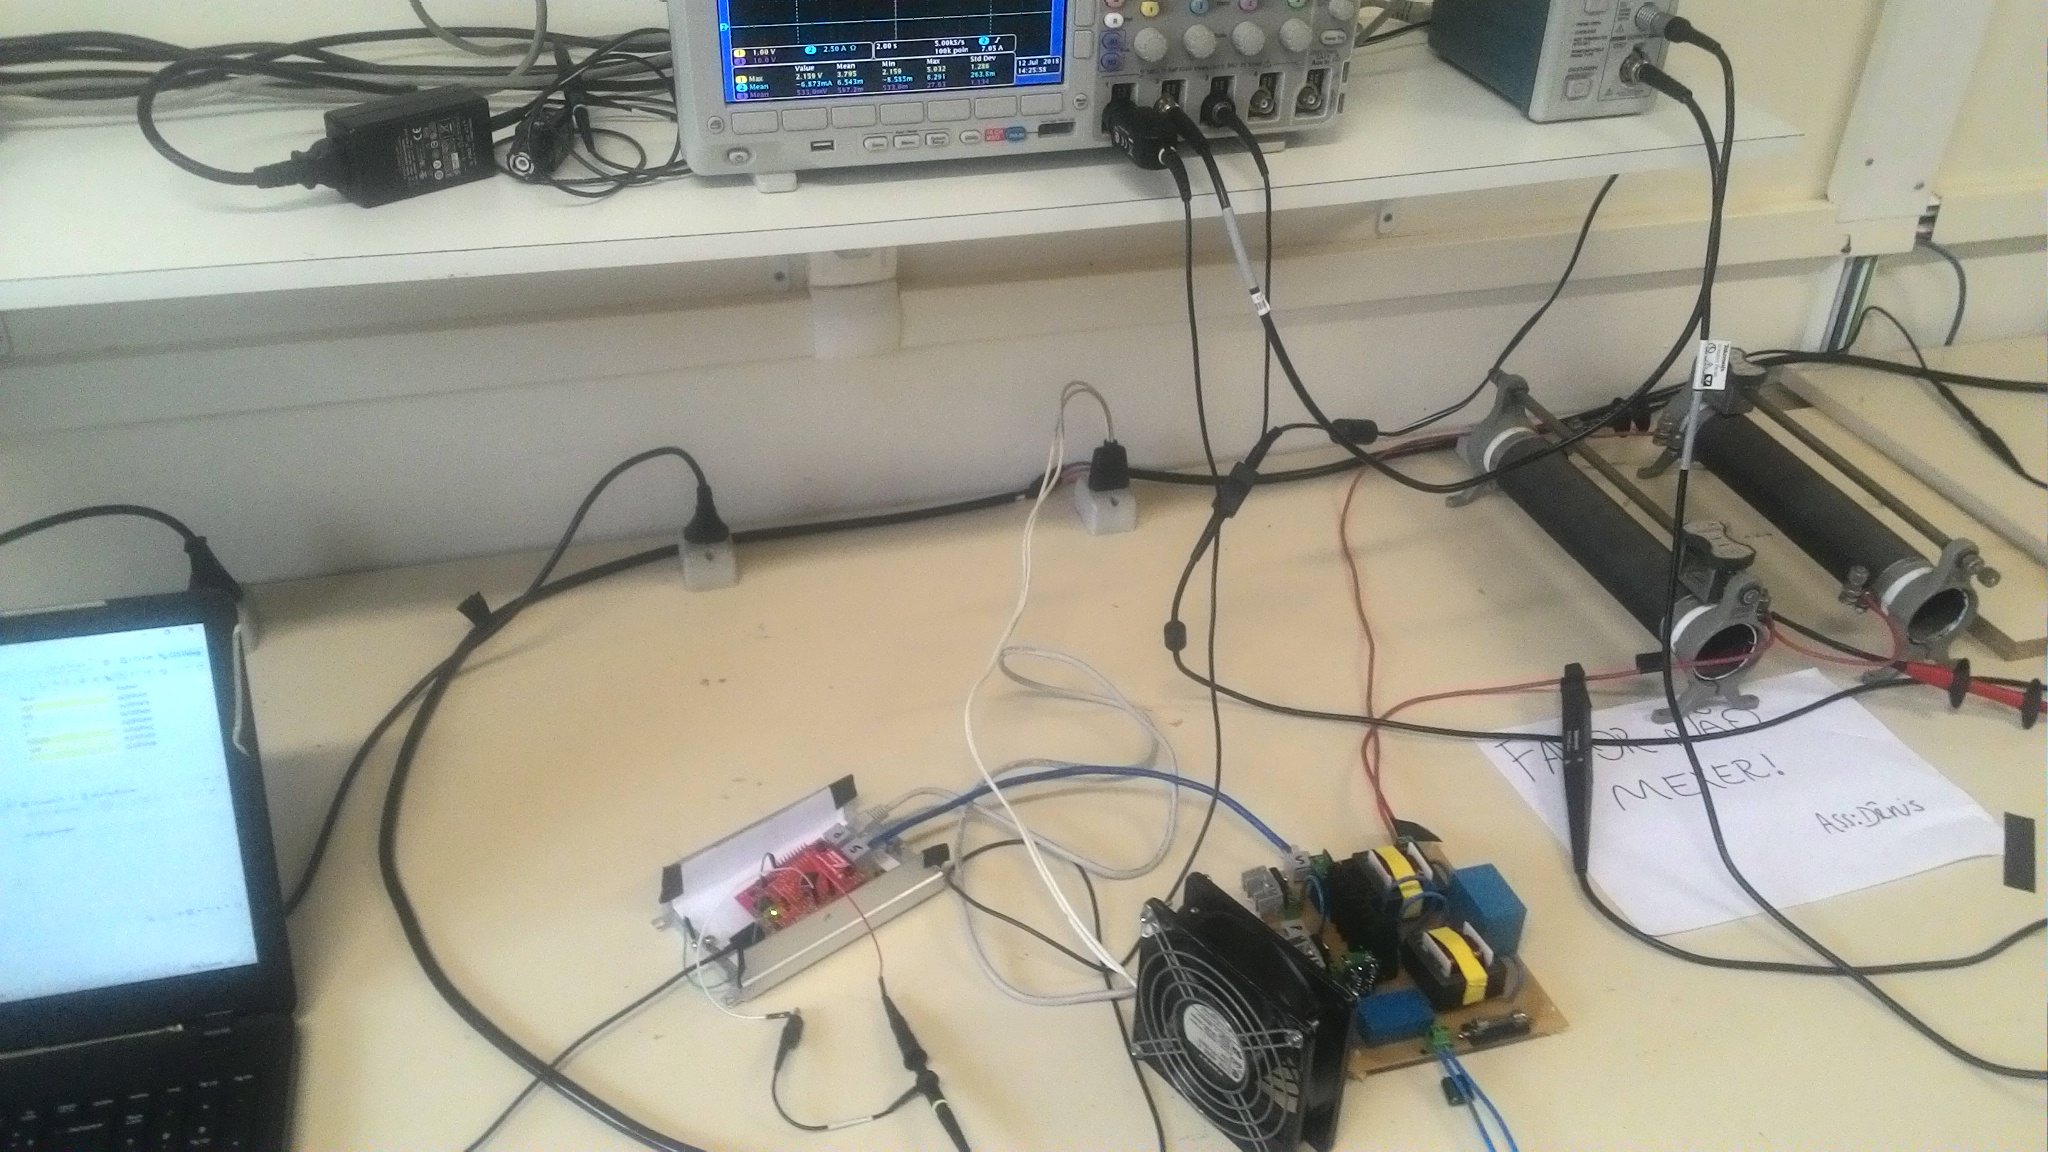
\includegraphics[height=2cm]{../../FOTOGRAFIAS/P_20180712_152422.jpg}}\qquad
			\subfigure[Placa de potência.]{
				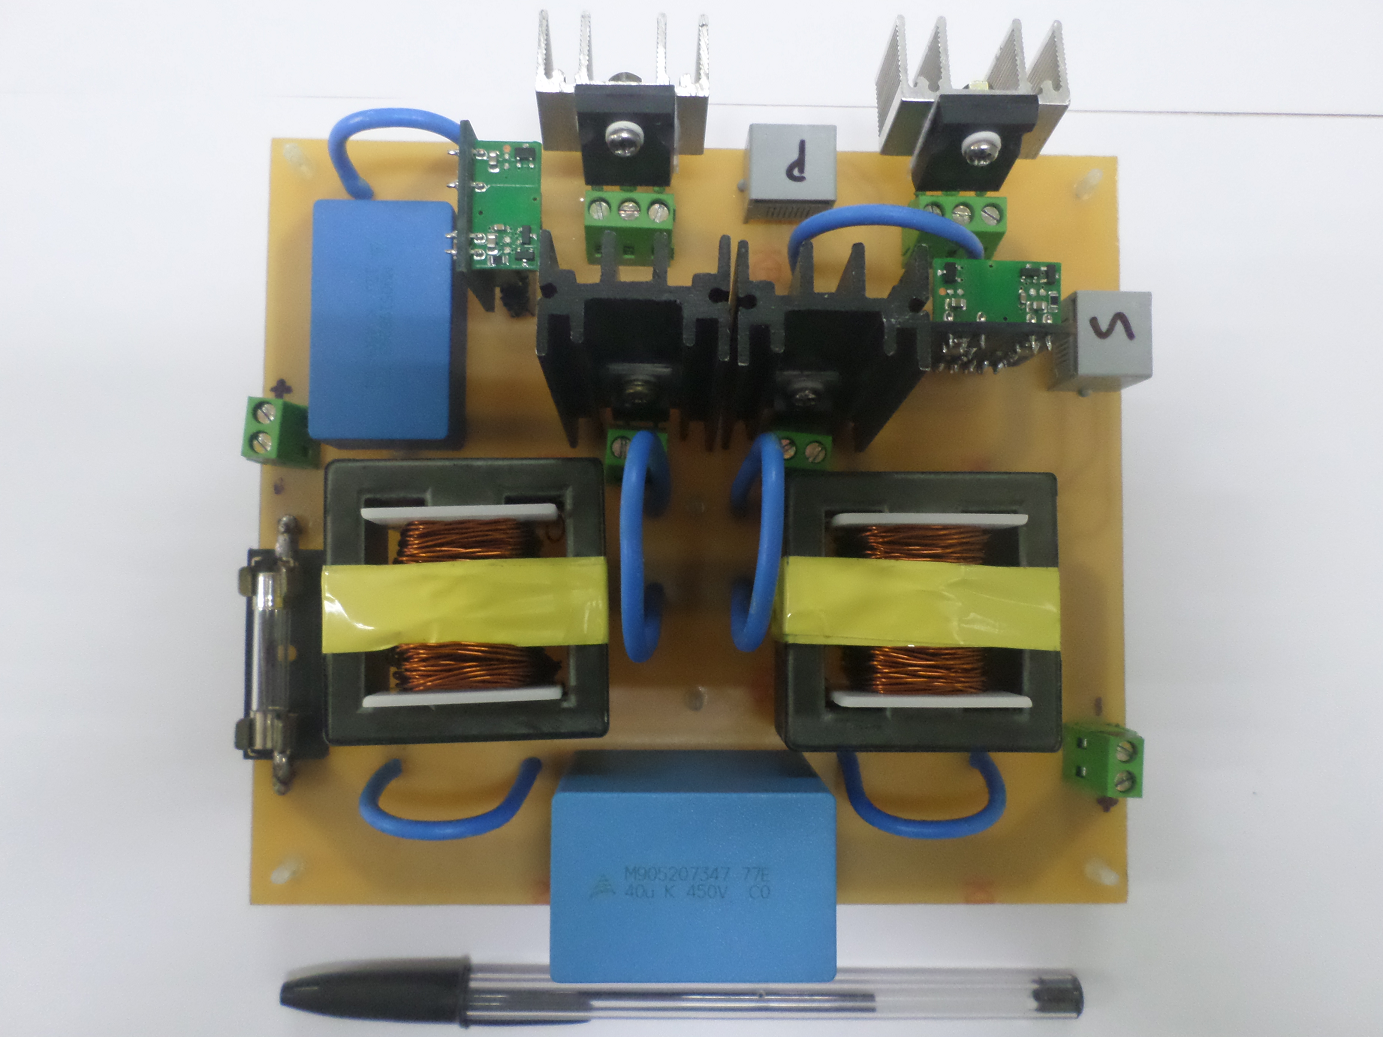
\includegraphics[height=2cm]{../../FOTOGRAFIAS/D1.png}}
		}
		\mbox{
			\subfigure[Sensoreamento de corrente.]{
				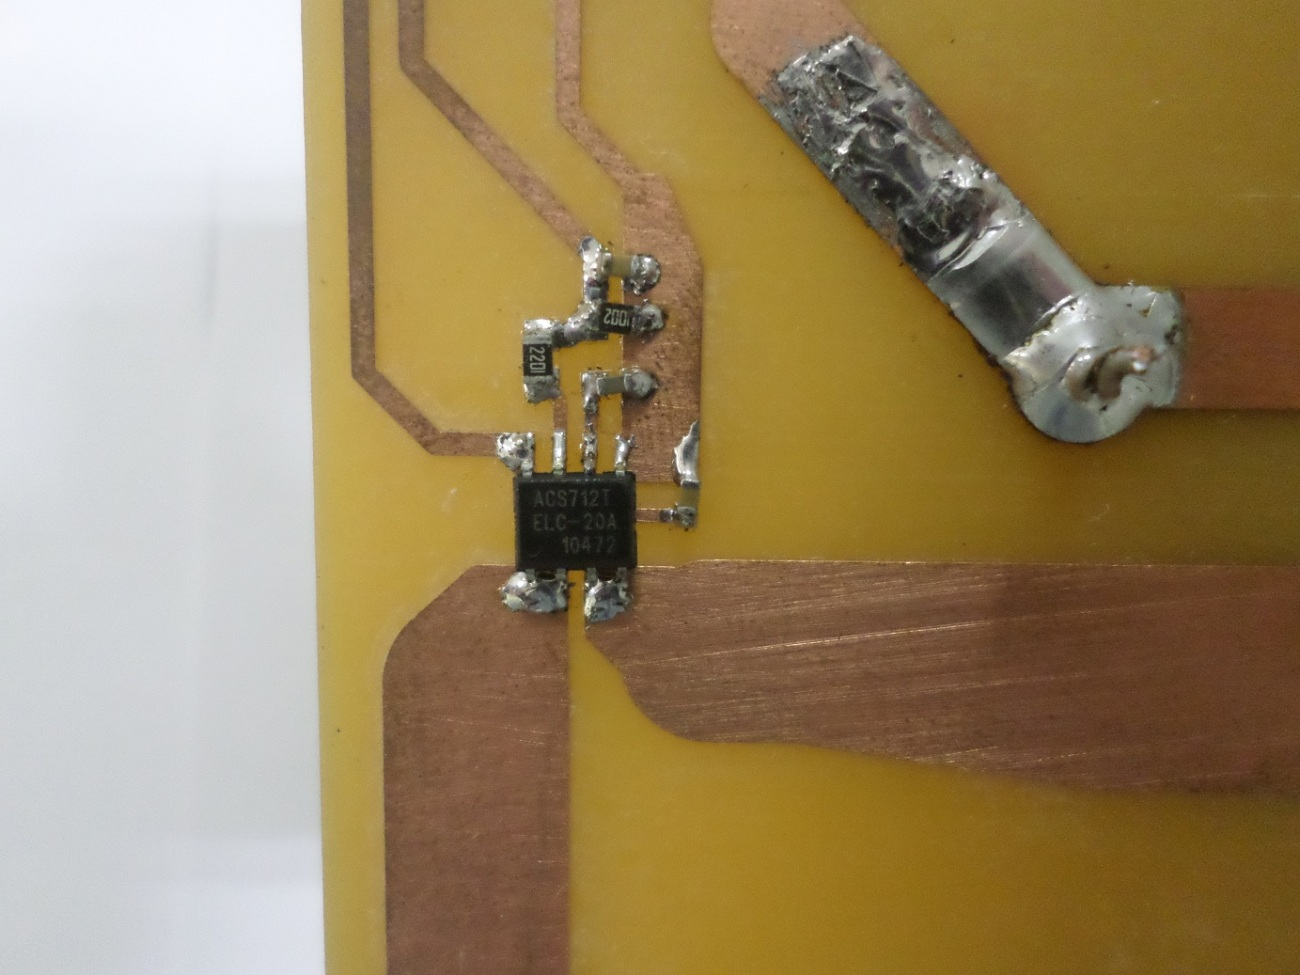
\includegraphics[height=2cm]{../../FOTOGRAFIAS/D2.jpg}}\qquad
			\subfigure[Tiva conectado à dock.]{
				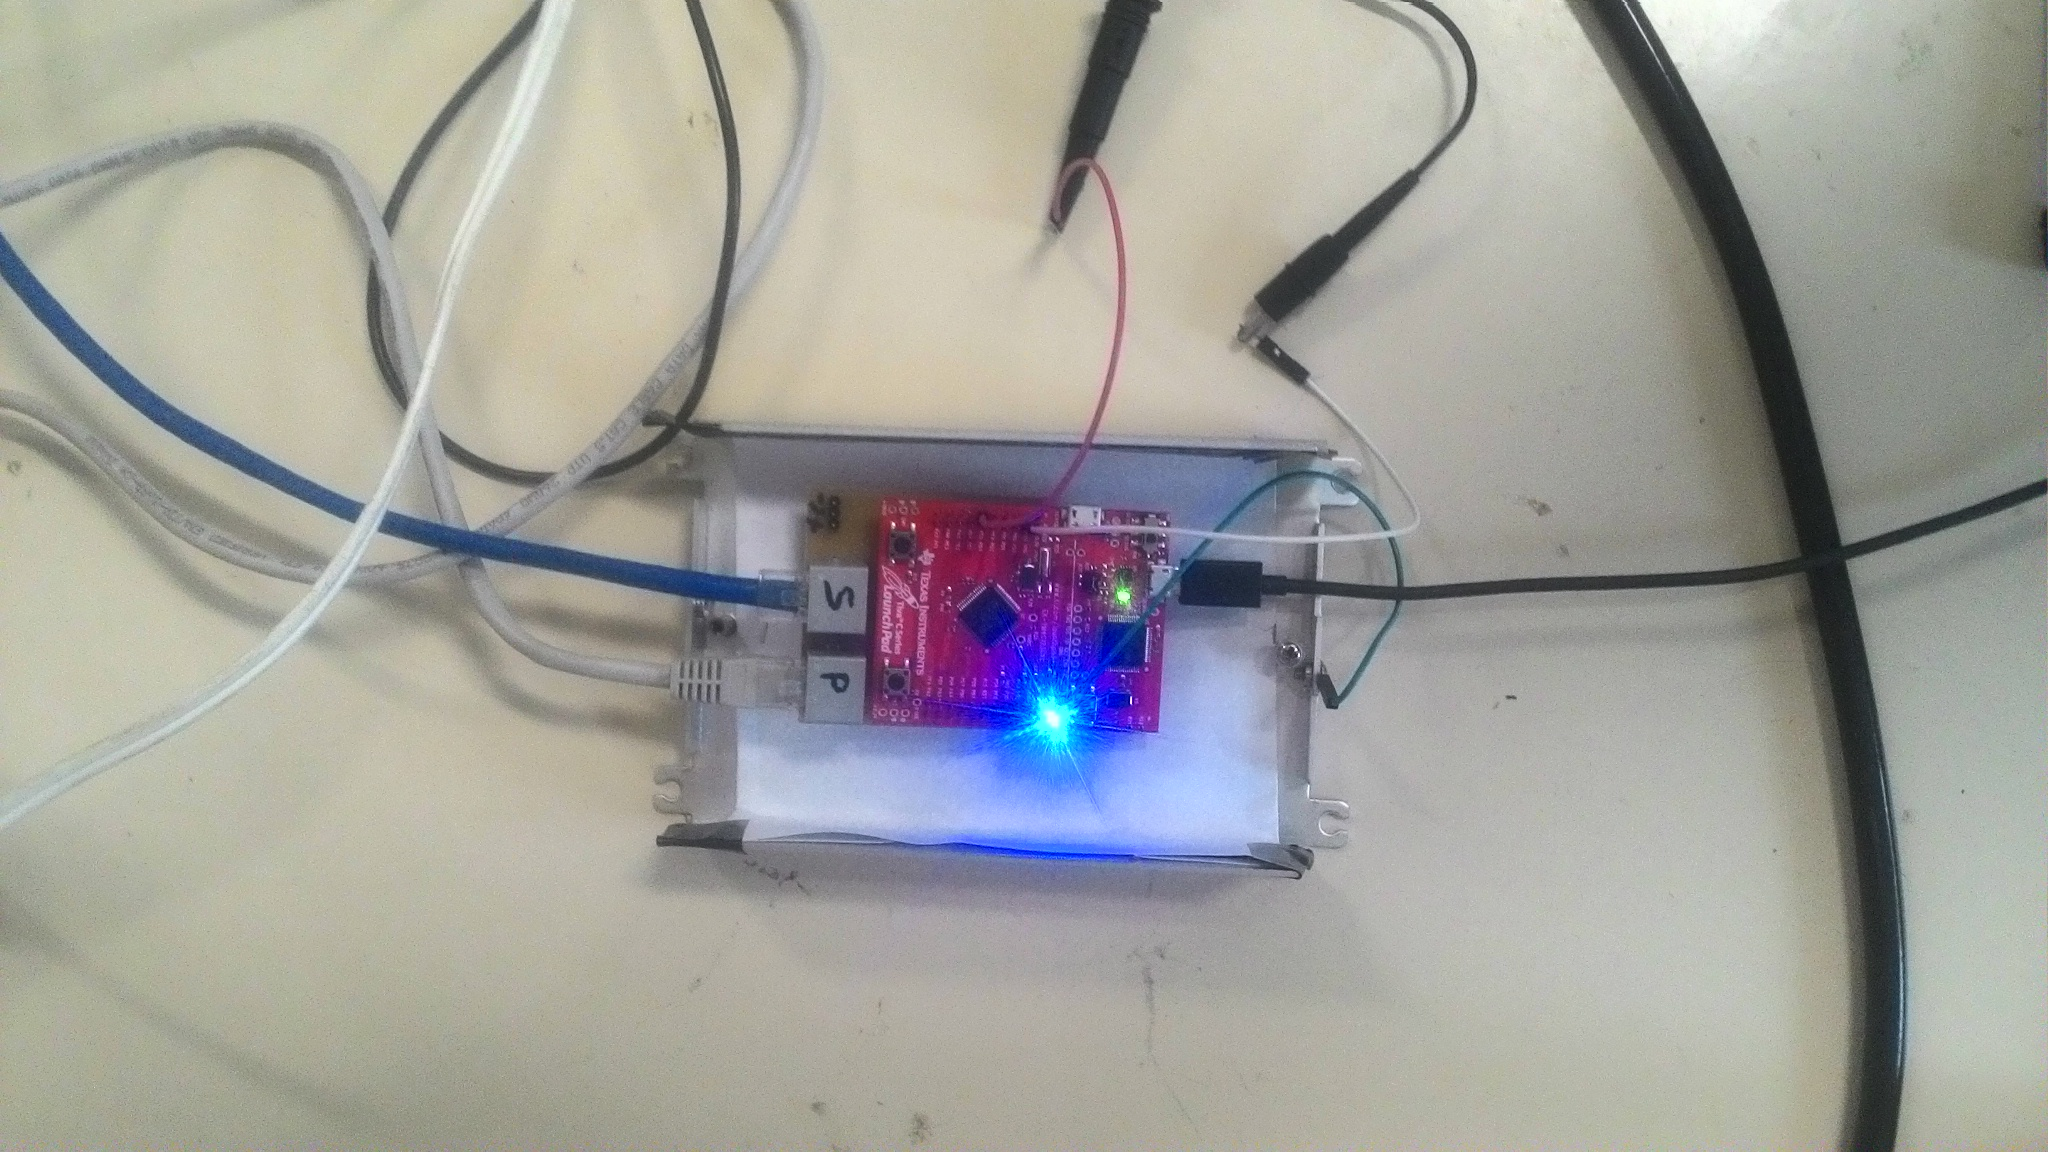
\includegraphics[height=2cm]{../../FOTOGRAFIAS/P_20180712_152414.jpg}}
		}
	\end{figure}
\end{frame}
%----------------------------------------------------------
\subsection{Resultados práticos}
\begin{frame}{Formas de onda do barramento}
	\begin{figure}[htb]
		\centering
		\mbox{
			\subfigure[Tensão e corrente de entrada em 220V.]{
				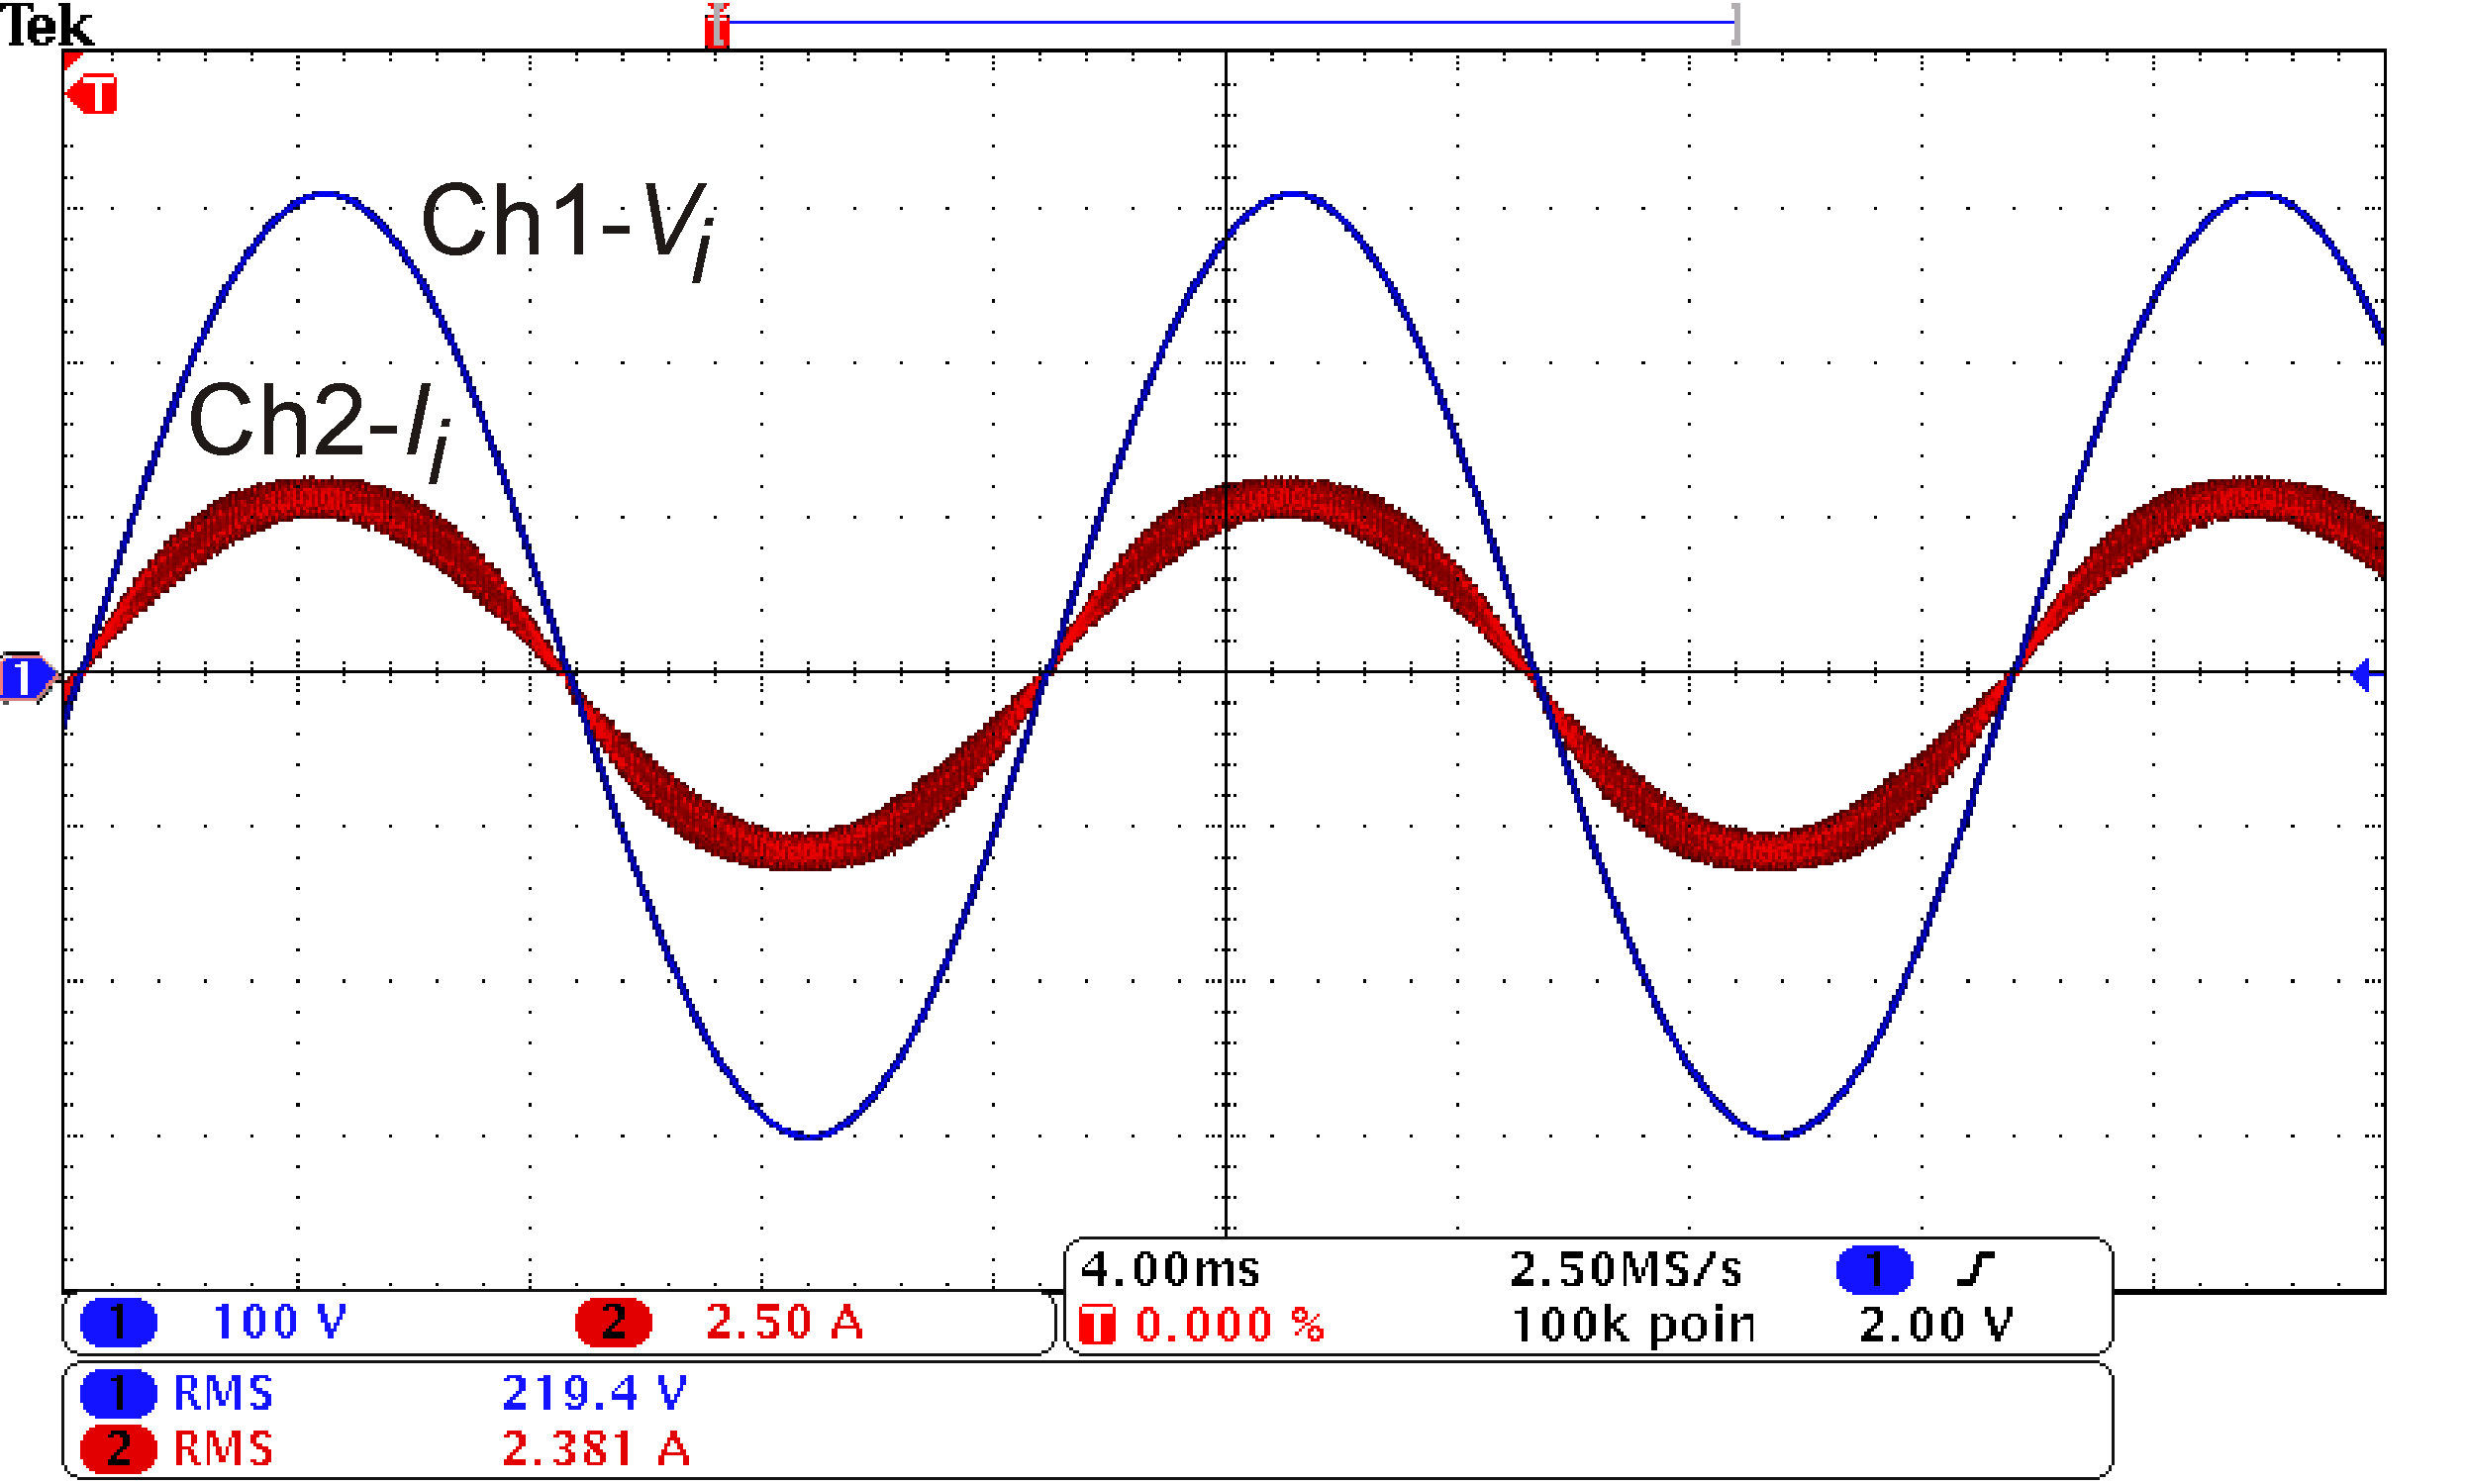
\includegraphics[height=3cm]{../../FIGURAS/Figuras_TFC_Eric/Formas_de_onda/PFC_ACM}}\qquad
			\subfigure[Tensão e corrente de entrada em 127V.]{
				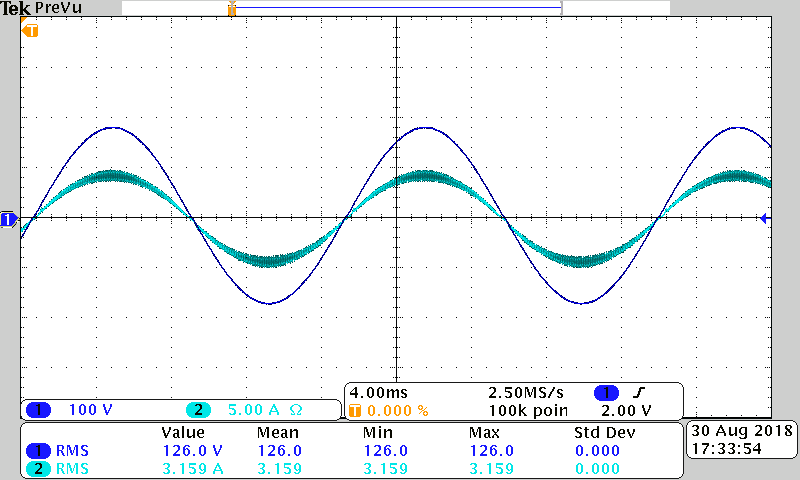
\includegraphics[height=3cm]{../../GRAFICOS/TEK/tek00042}}
		}
	\end{figure}
\end{frame}
%----------------------------------------------------------
\begin{frame}{Formas de onda do barramento}
	\begin{figure}[htb]
		\centering
		\mbox{
			\subfigure[Corrente no indutor e tensão no barramento.]{
				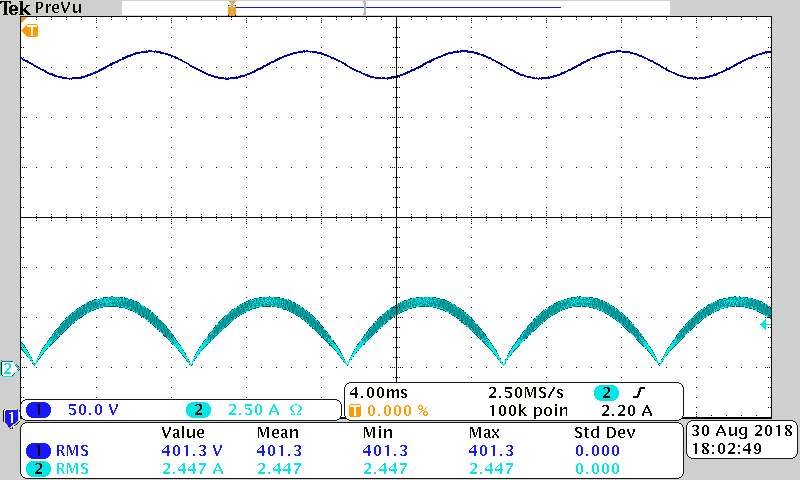
\includegraphics[height=3cm]{../../GRAFICOS/TEK/tek00064}}\qquad
			\subfigure[Distúrbio na entrada.]{
				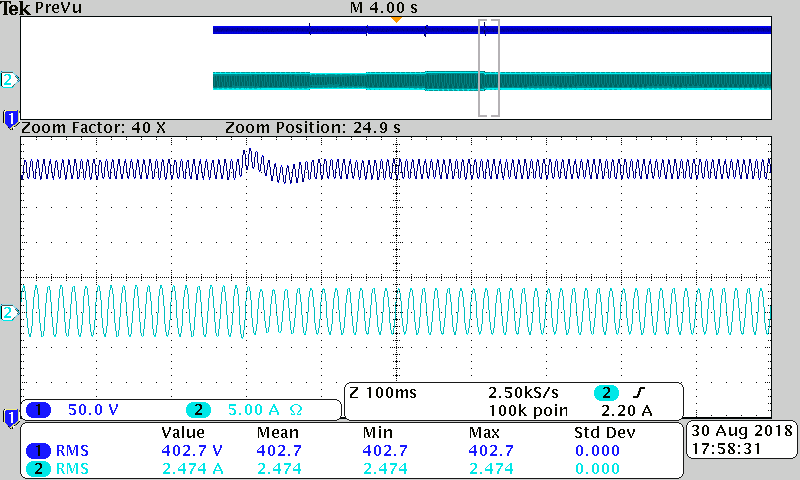
\includegraphics[height=3cm]{../../GRAFICOS/TEK/tek00058}}
		}
	\end{figure}
\end{frame}
%----------------------------------------------------------
\begin{frame}{Formas de onda do segundo estágio}
	\begin{figure}[htb]
		\centering
		\mbox{
			\subfigure[Corrente e tensão nos diodos.]{
				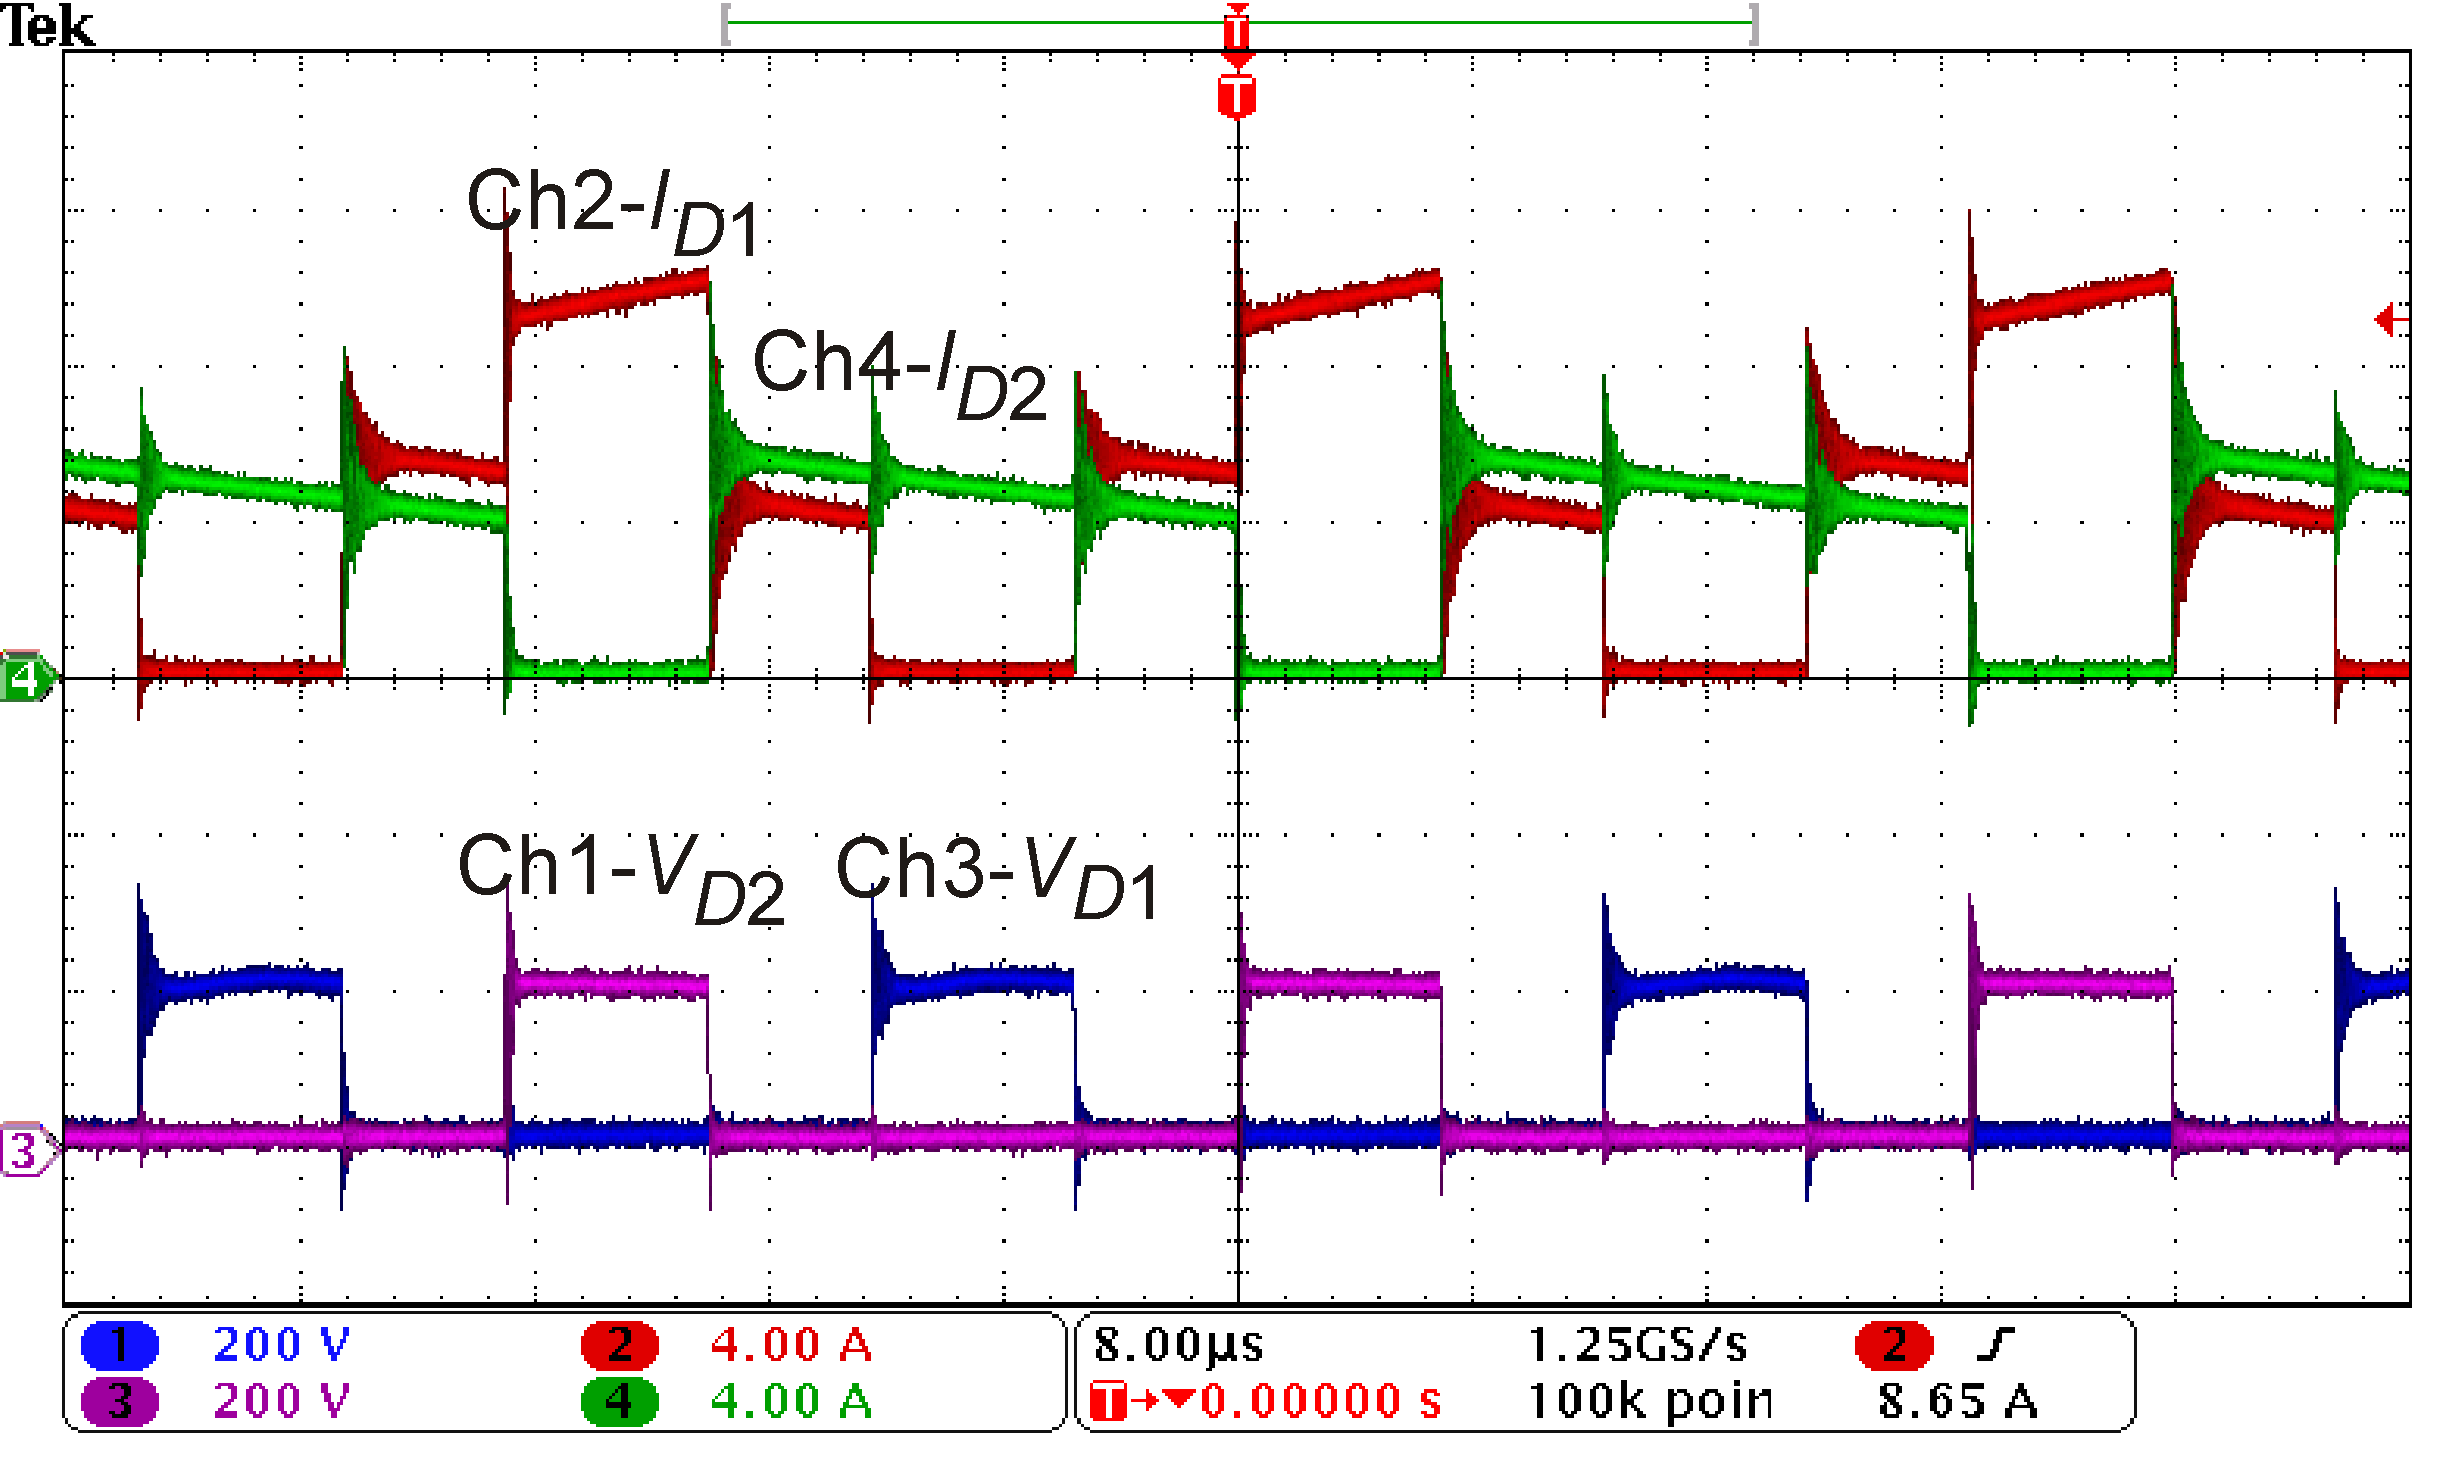
\includegraphics[height=3cm]{../../FIGURAS/Figuras_TFC_Eric/Formas_de_onda/Diodos_EGIBC}}\qquad
			\subfigure[Corrente e tensão nas chaves.]{
				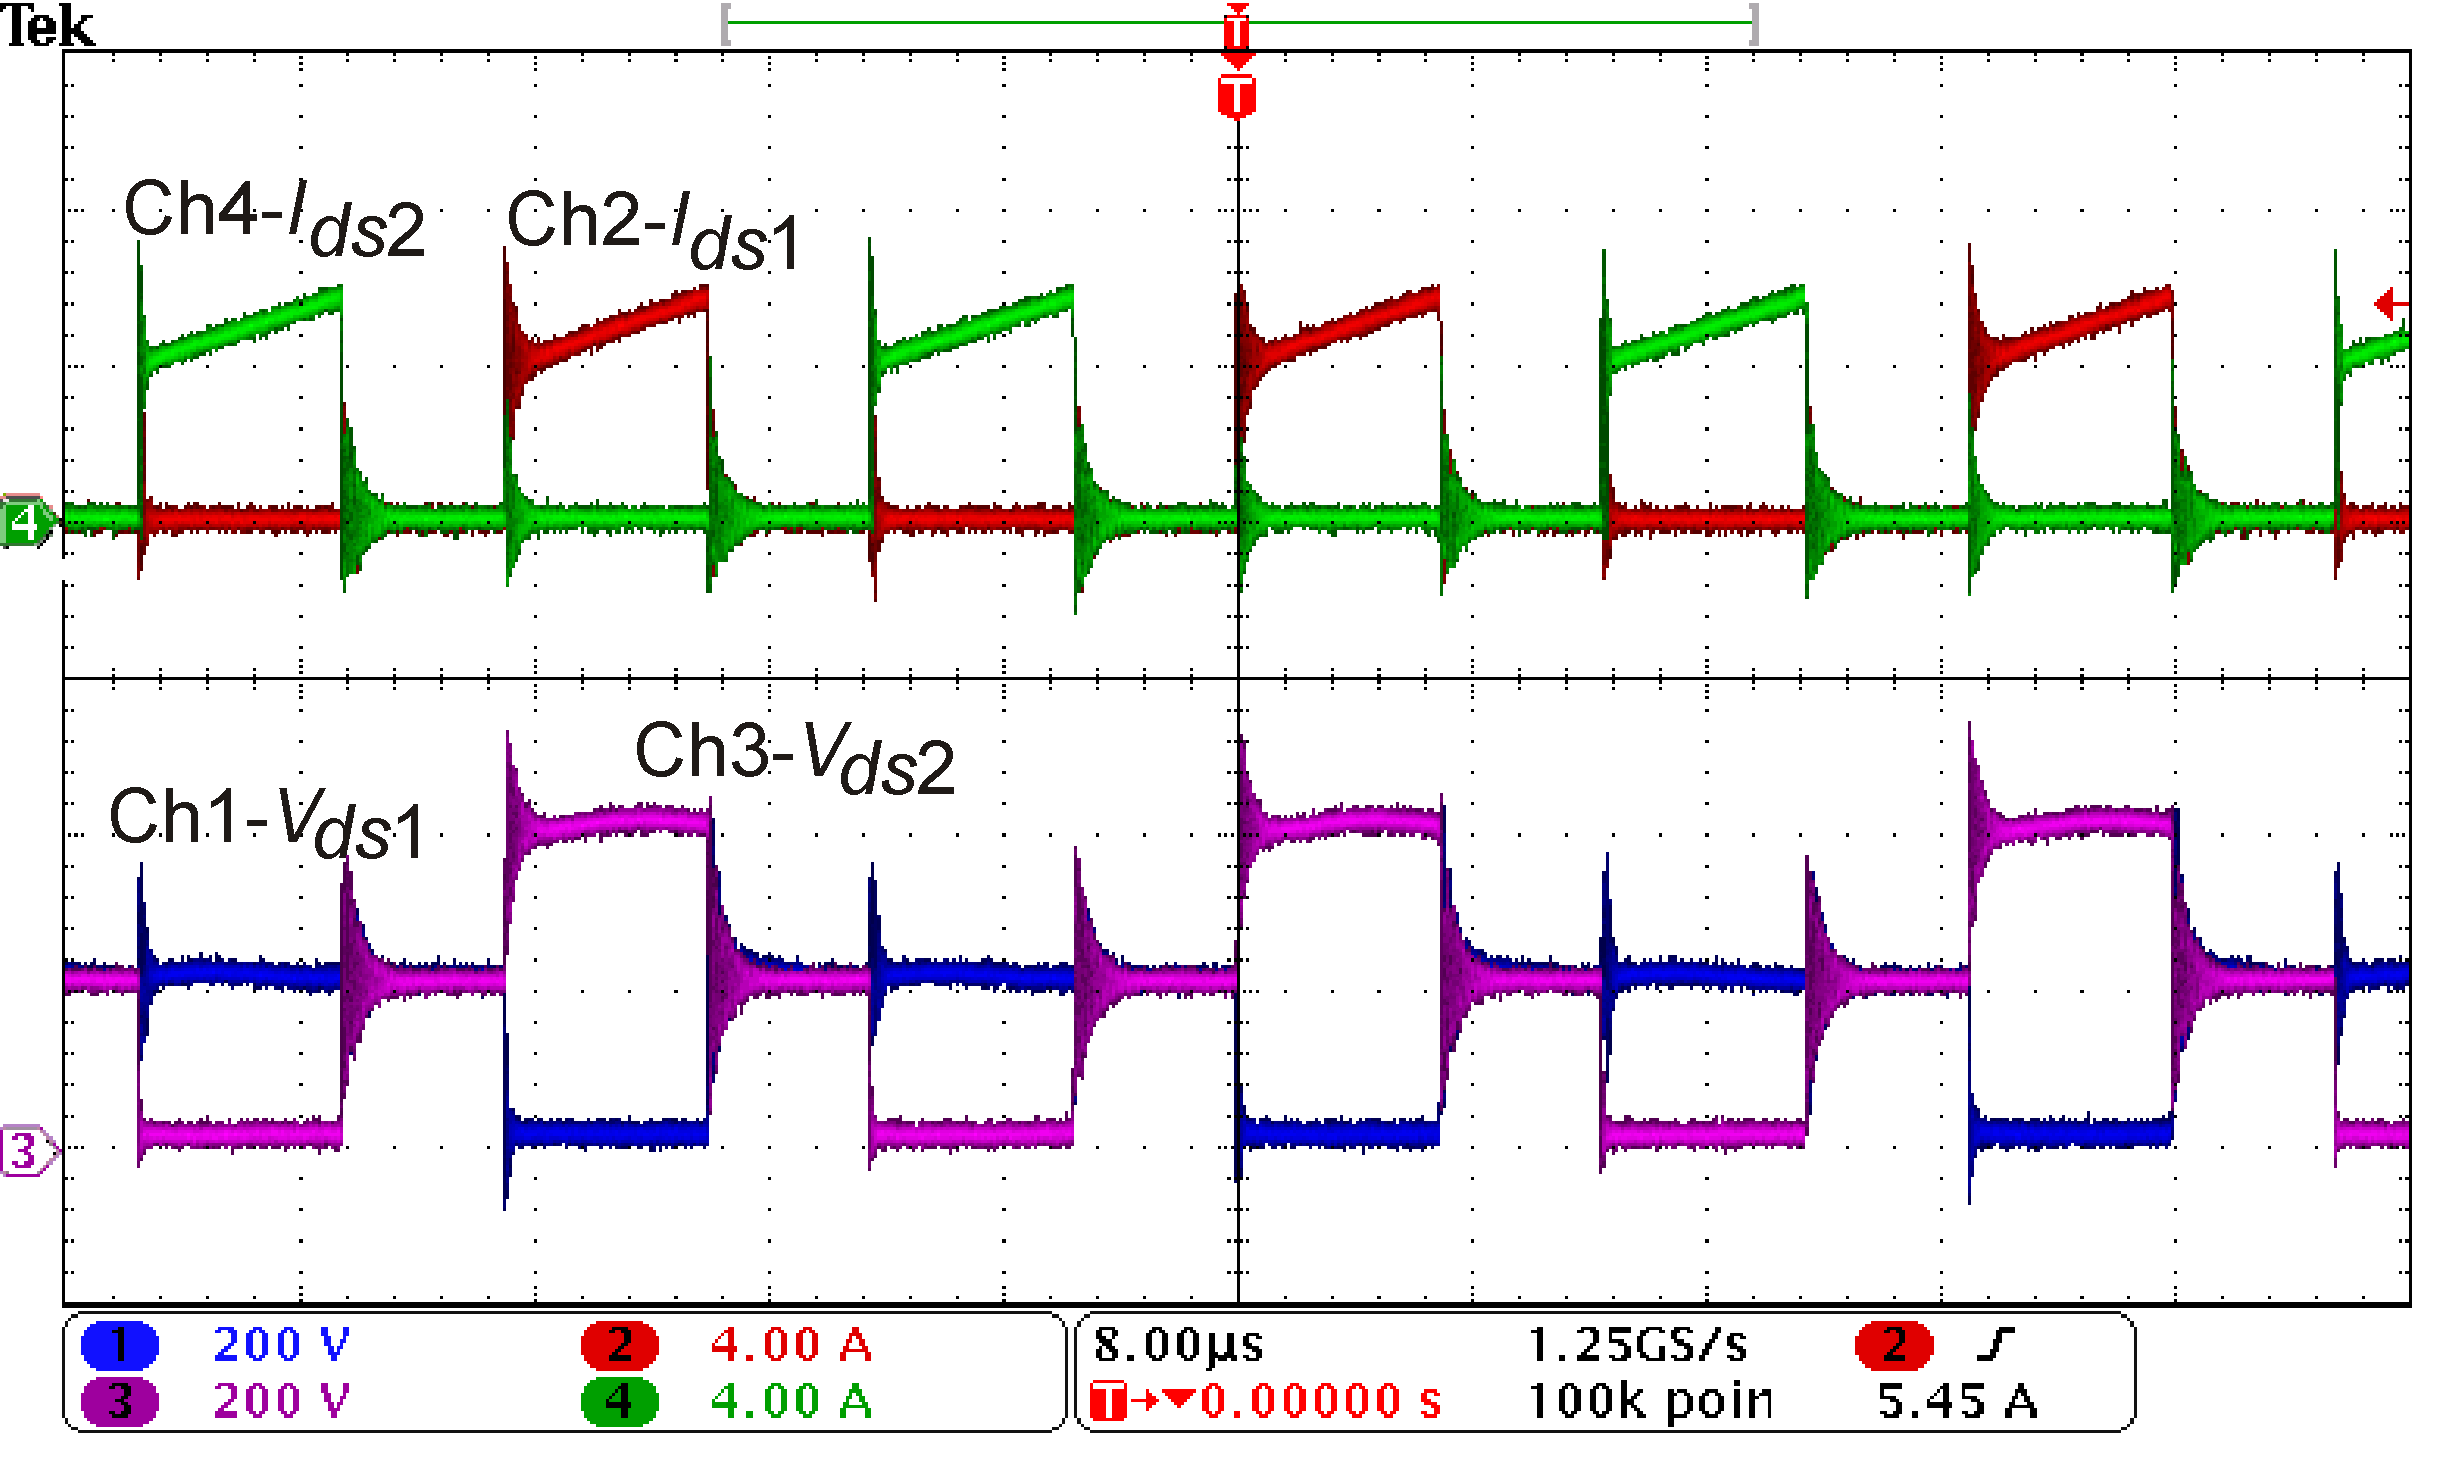
\includegraphics[height=3cm]{../../FIGURAS/Figuras_TFC_Eric/Formas_de_onda/MOSFETs_EGIBC}}
		}
	\end{figure}
\end{frame}
%----------------------------------------------------------
\begin{frame}{Formas de onda do segundo estágio}
	\begin{figure}[htb]
		\centering
		\mbox{
			\subfigure[Corrente nos indutores e disparo das chaves.]{
				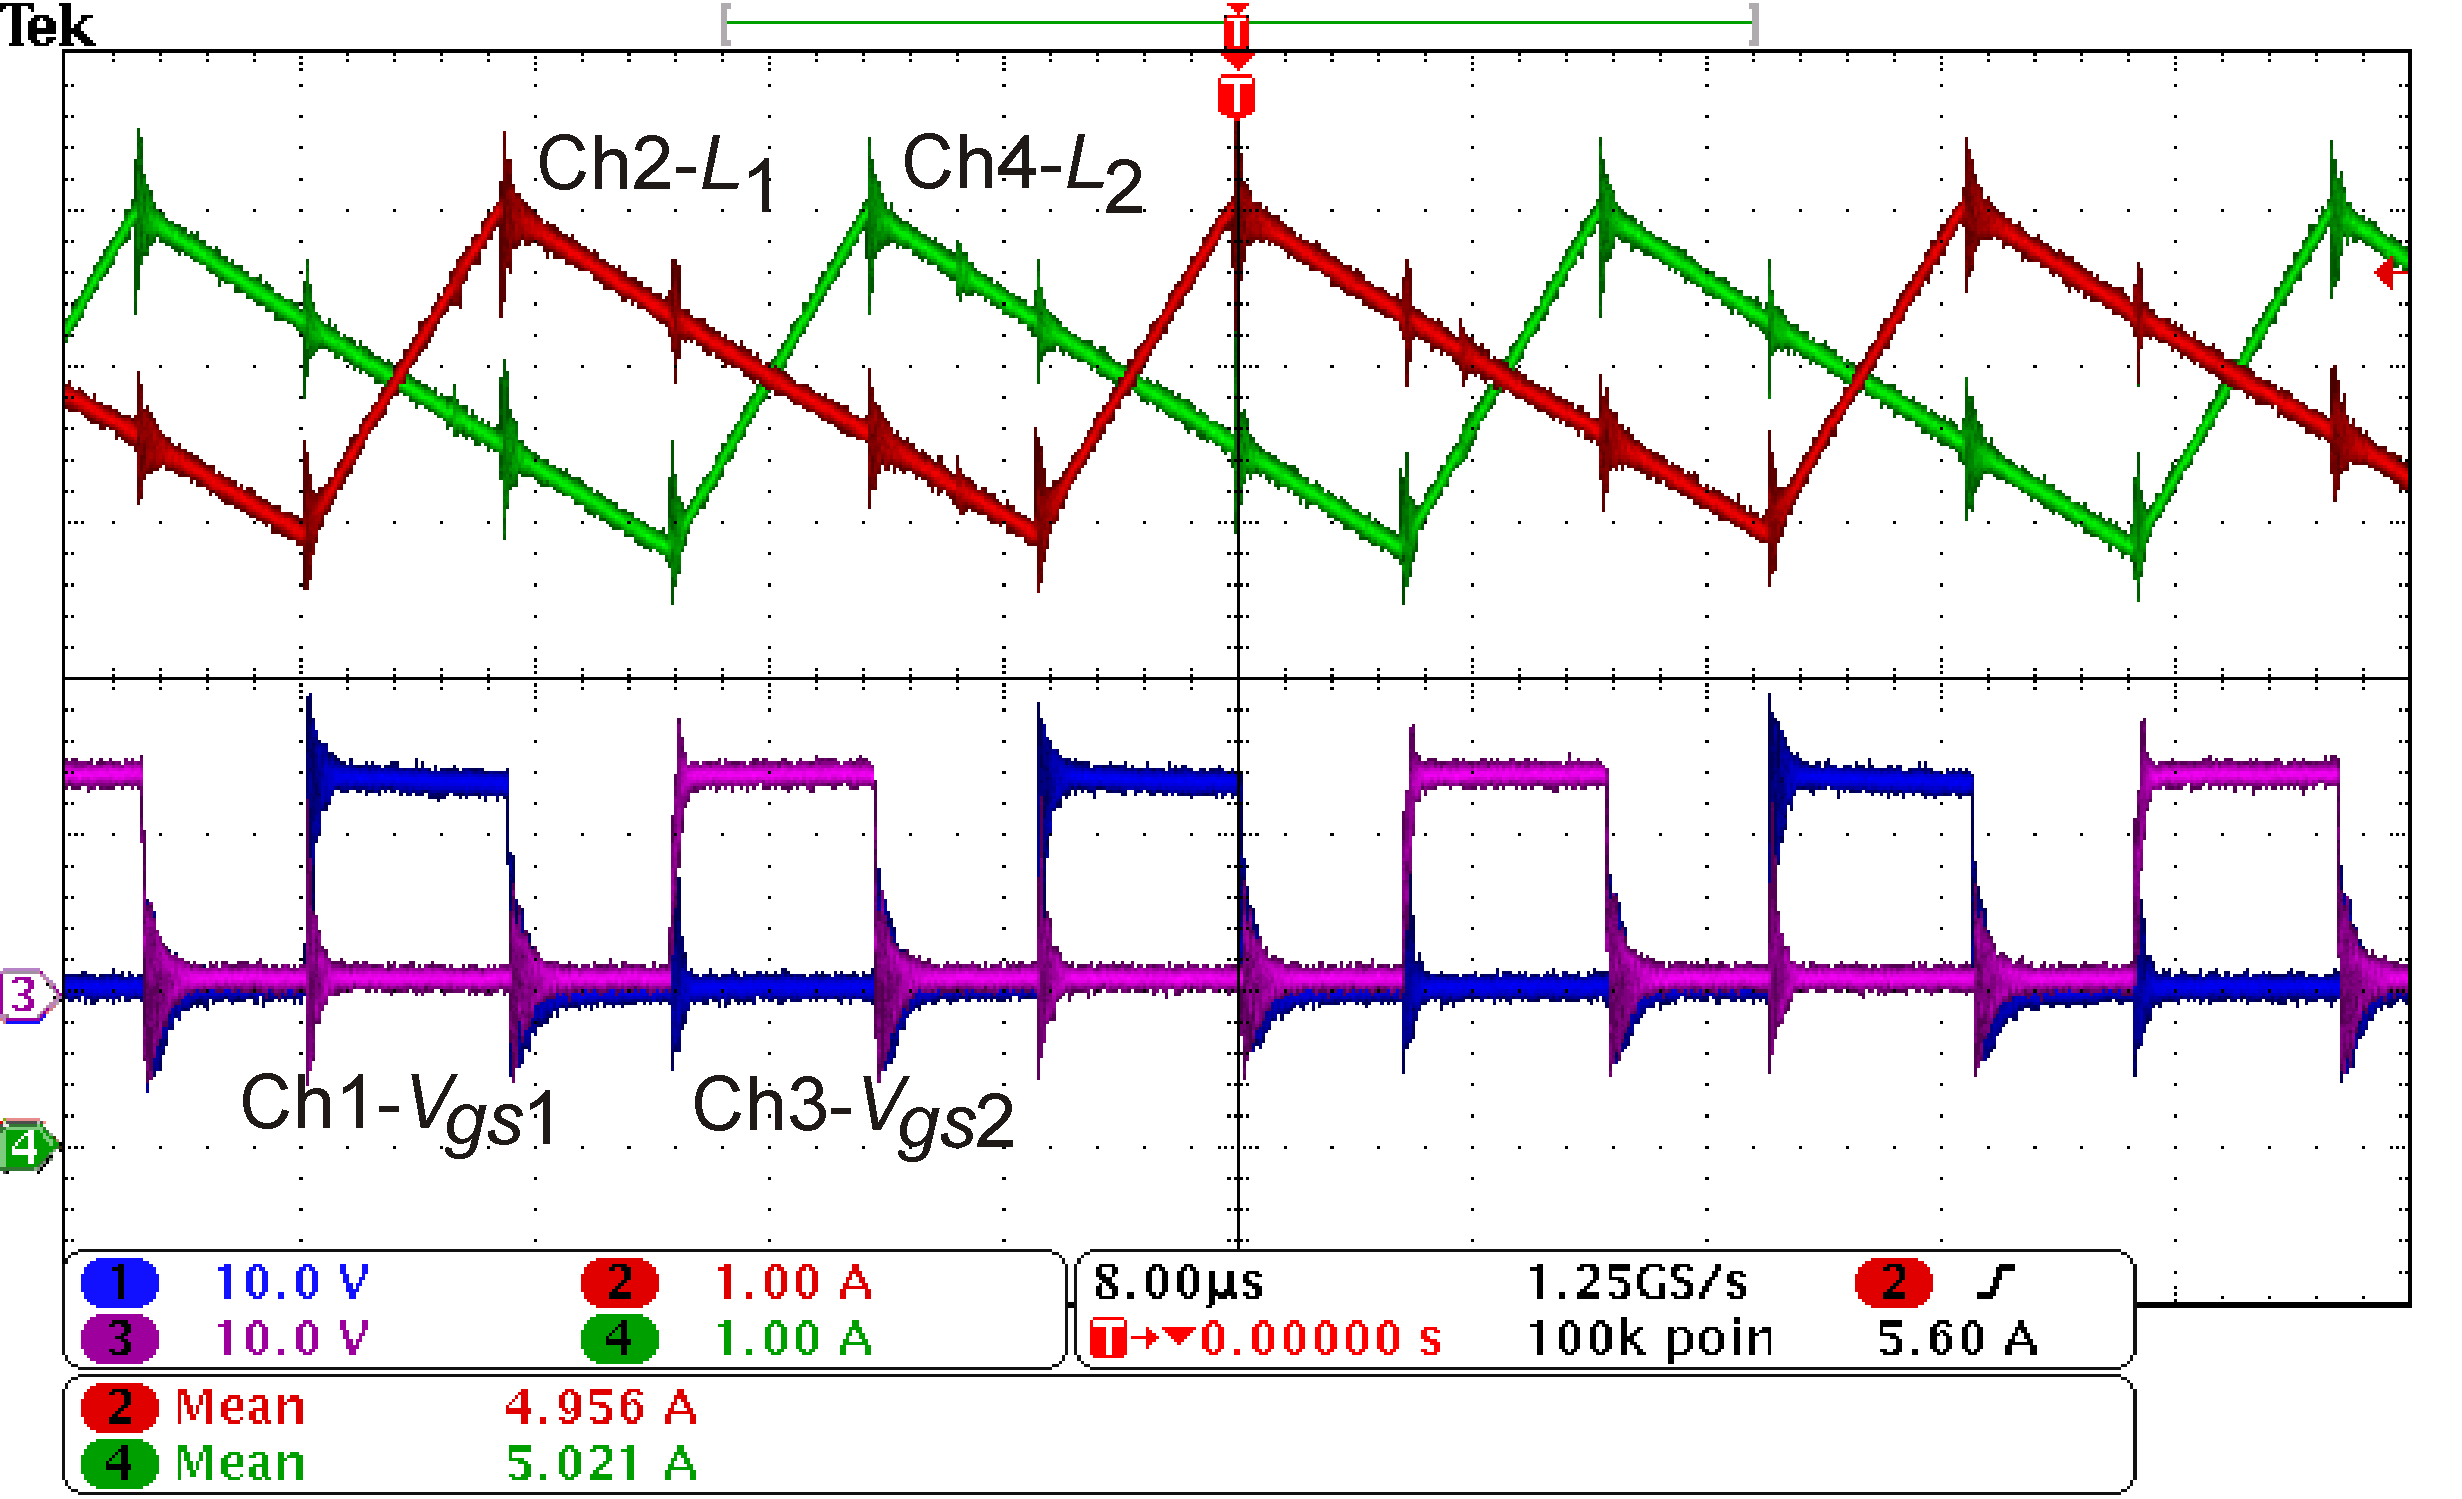
\includegraphics[height=3cm]{../../FIGURAS/Figuras_TFC_Eric/Formas_de_onda/Inductors_EGIBC}}\qquad
			\subfigure[Distúrbio no barramento.]{
				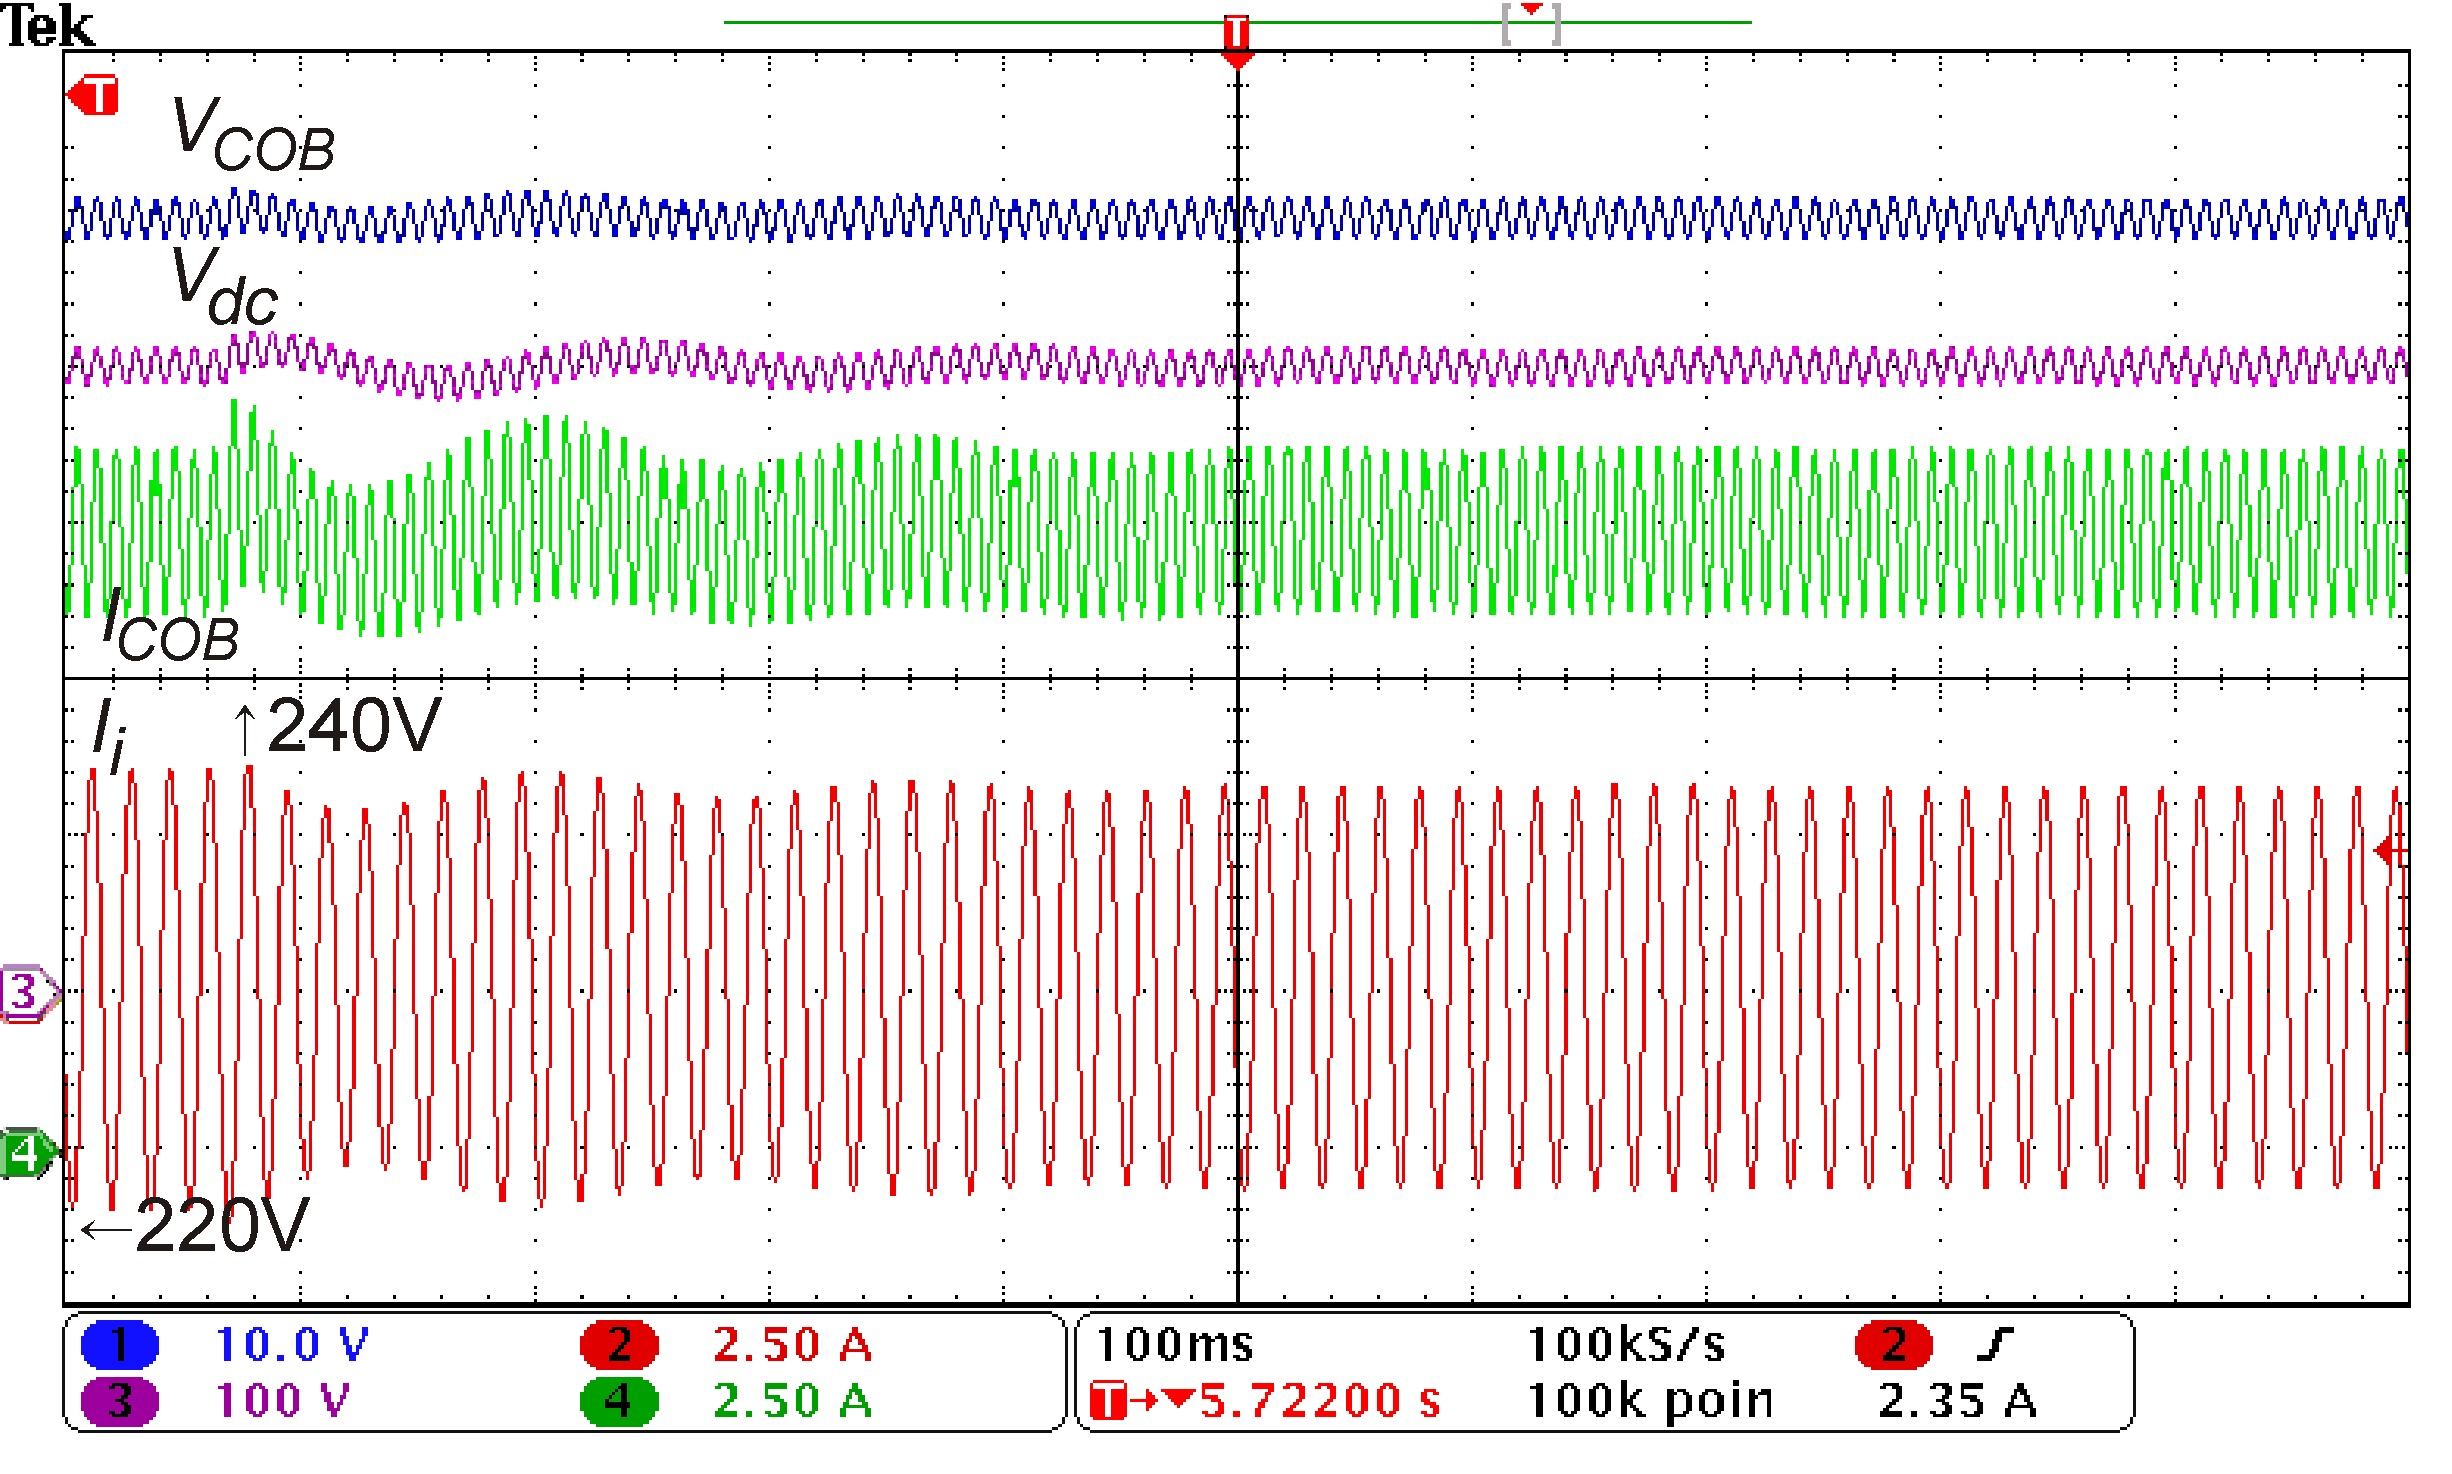
\includegraphics[height=3cm]{../../FIGURAS/Figuras_TFC_Eric/Formas_de_onda/Detailed_220V_to_240V}}
		}
	\end{figure}
\end{frame}
%----------------------------------------------------------
\begin{frame}{Resultados Gerais}
	\begin{figure}[htb]
		\centering
		\mbox{
			\subfigure[Dimerização do conversor.]{
				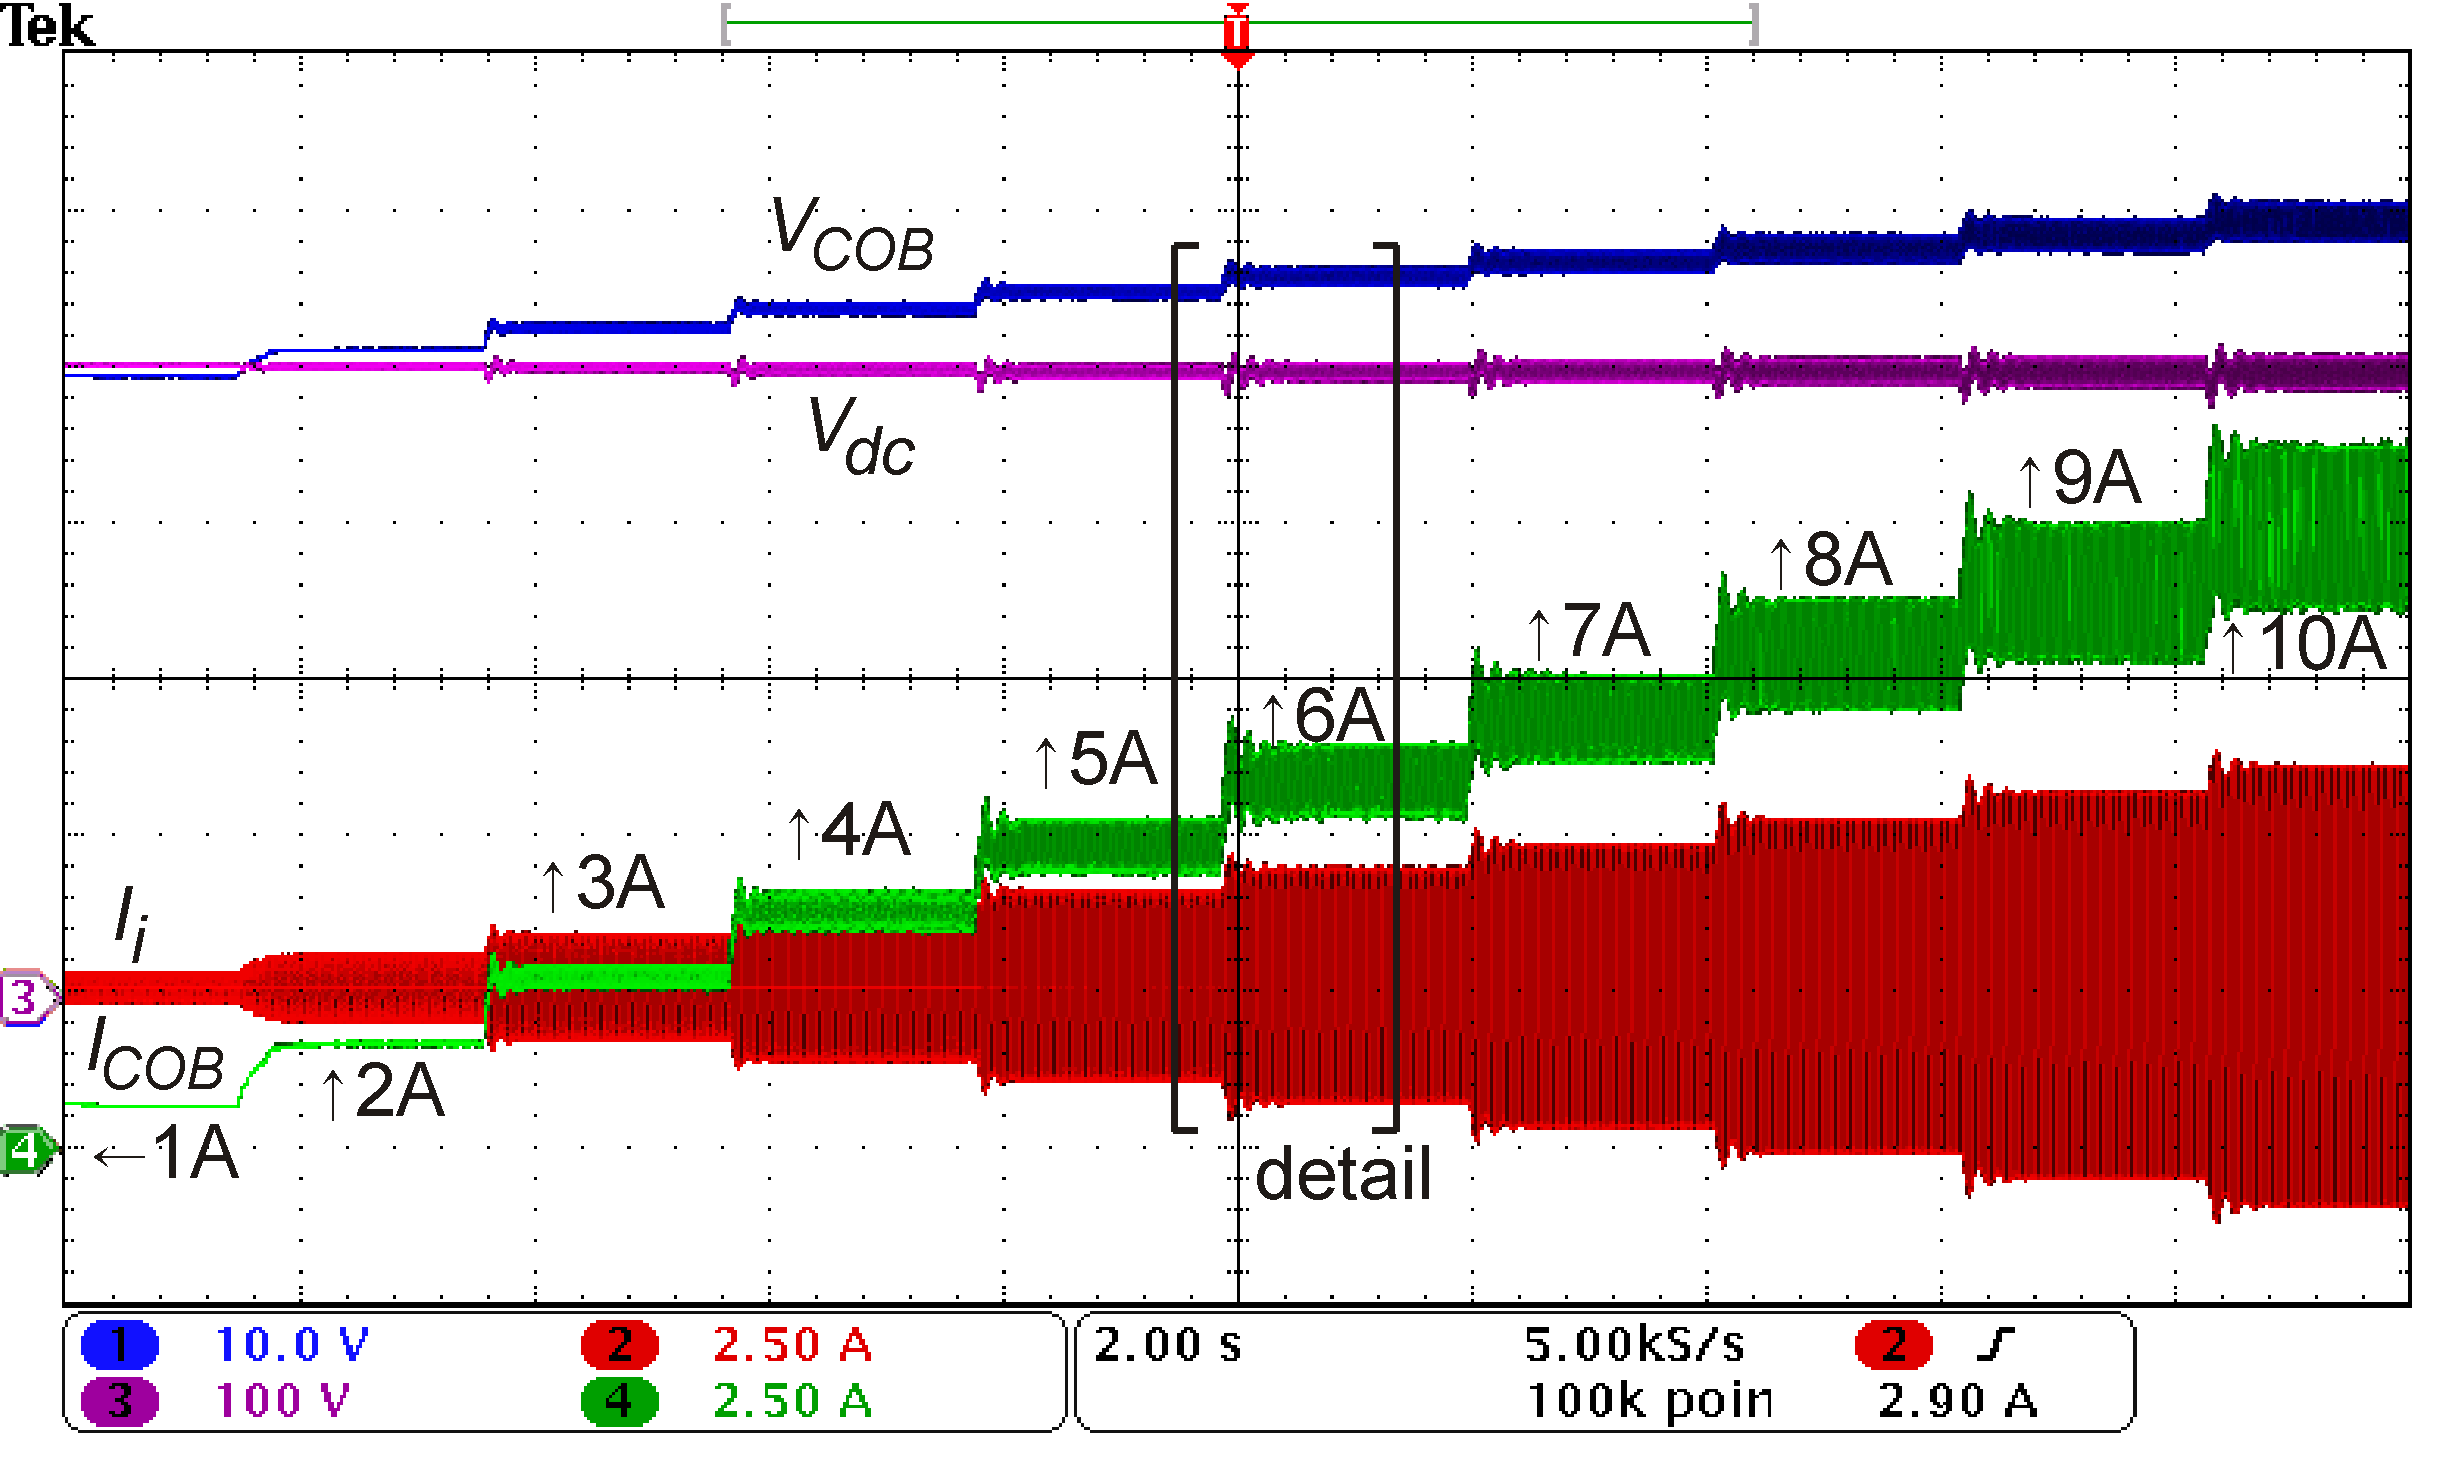
\includegraphics[height=3cm]{../../FIGURAS/Figuras_TFC_Eric/Formas_de_onda/Dimming}}\qquad
			\subfigure[Harmônicas sob máscara da IEC 61000-3-2 Classe C.]{
				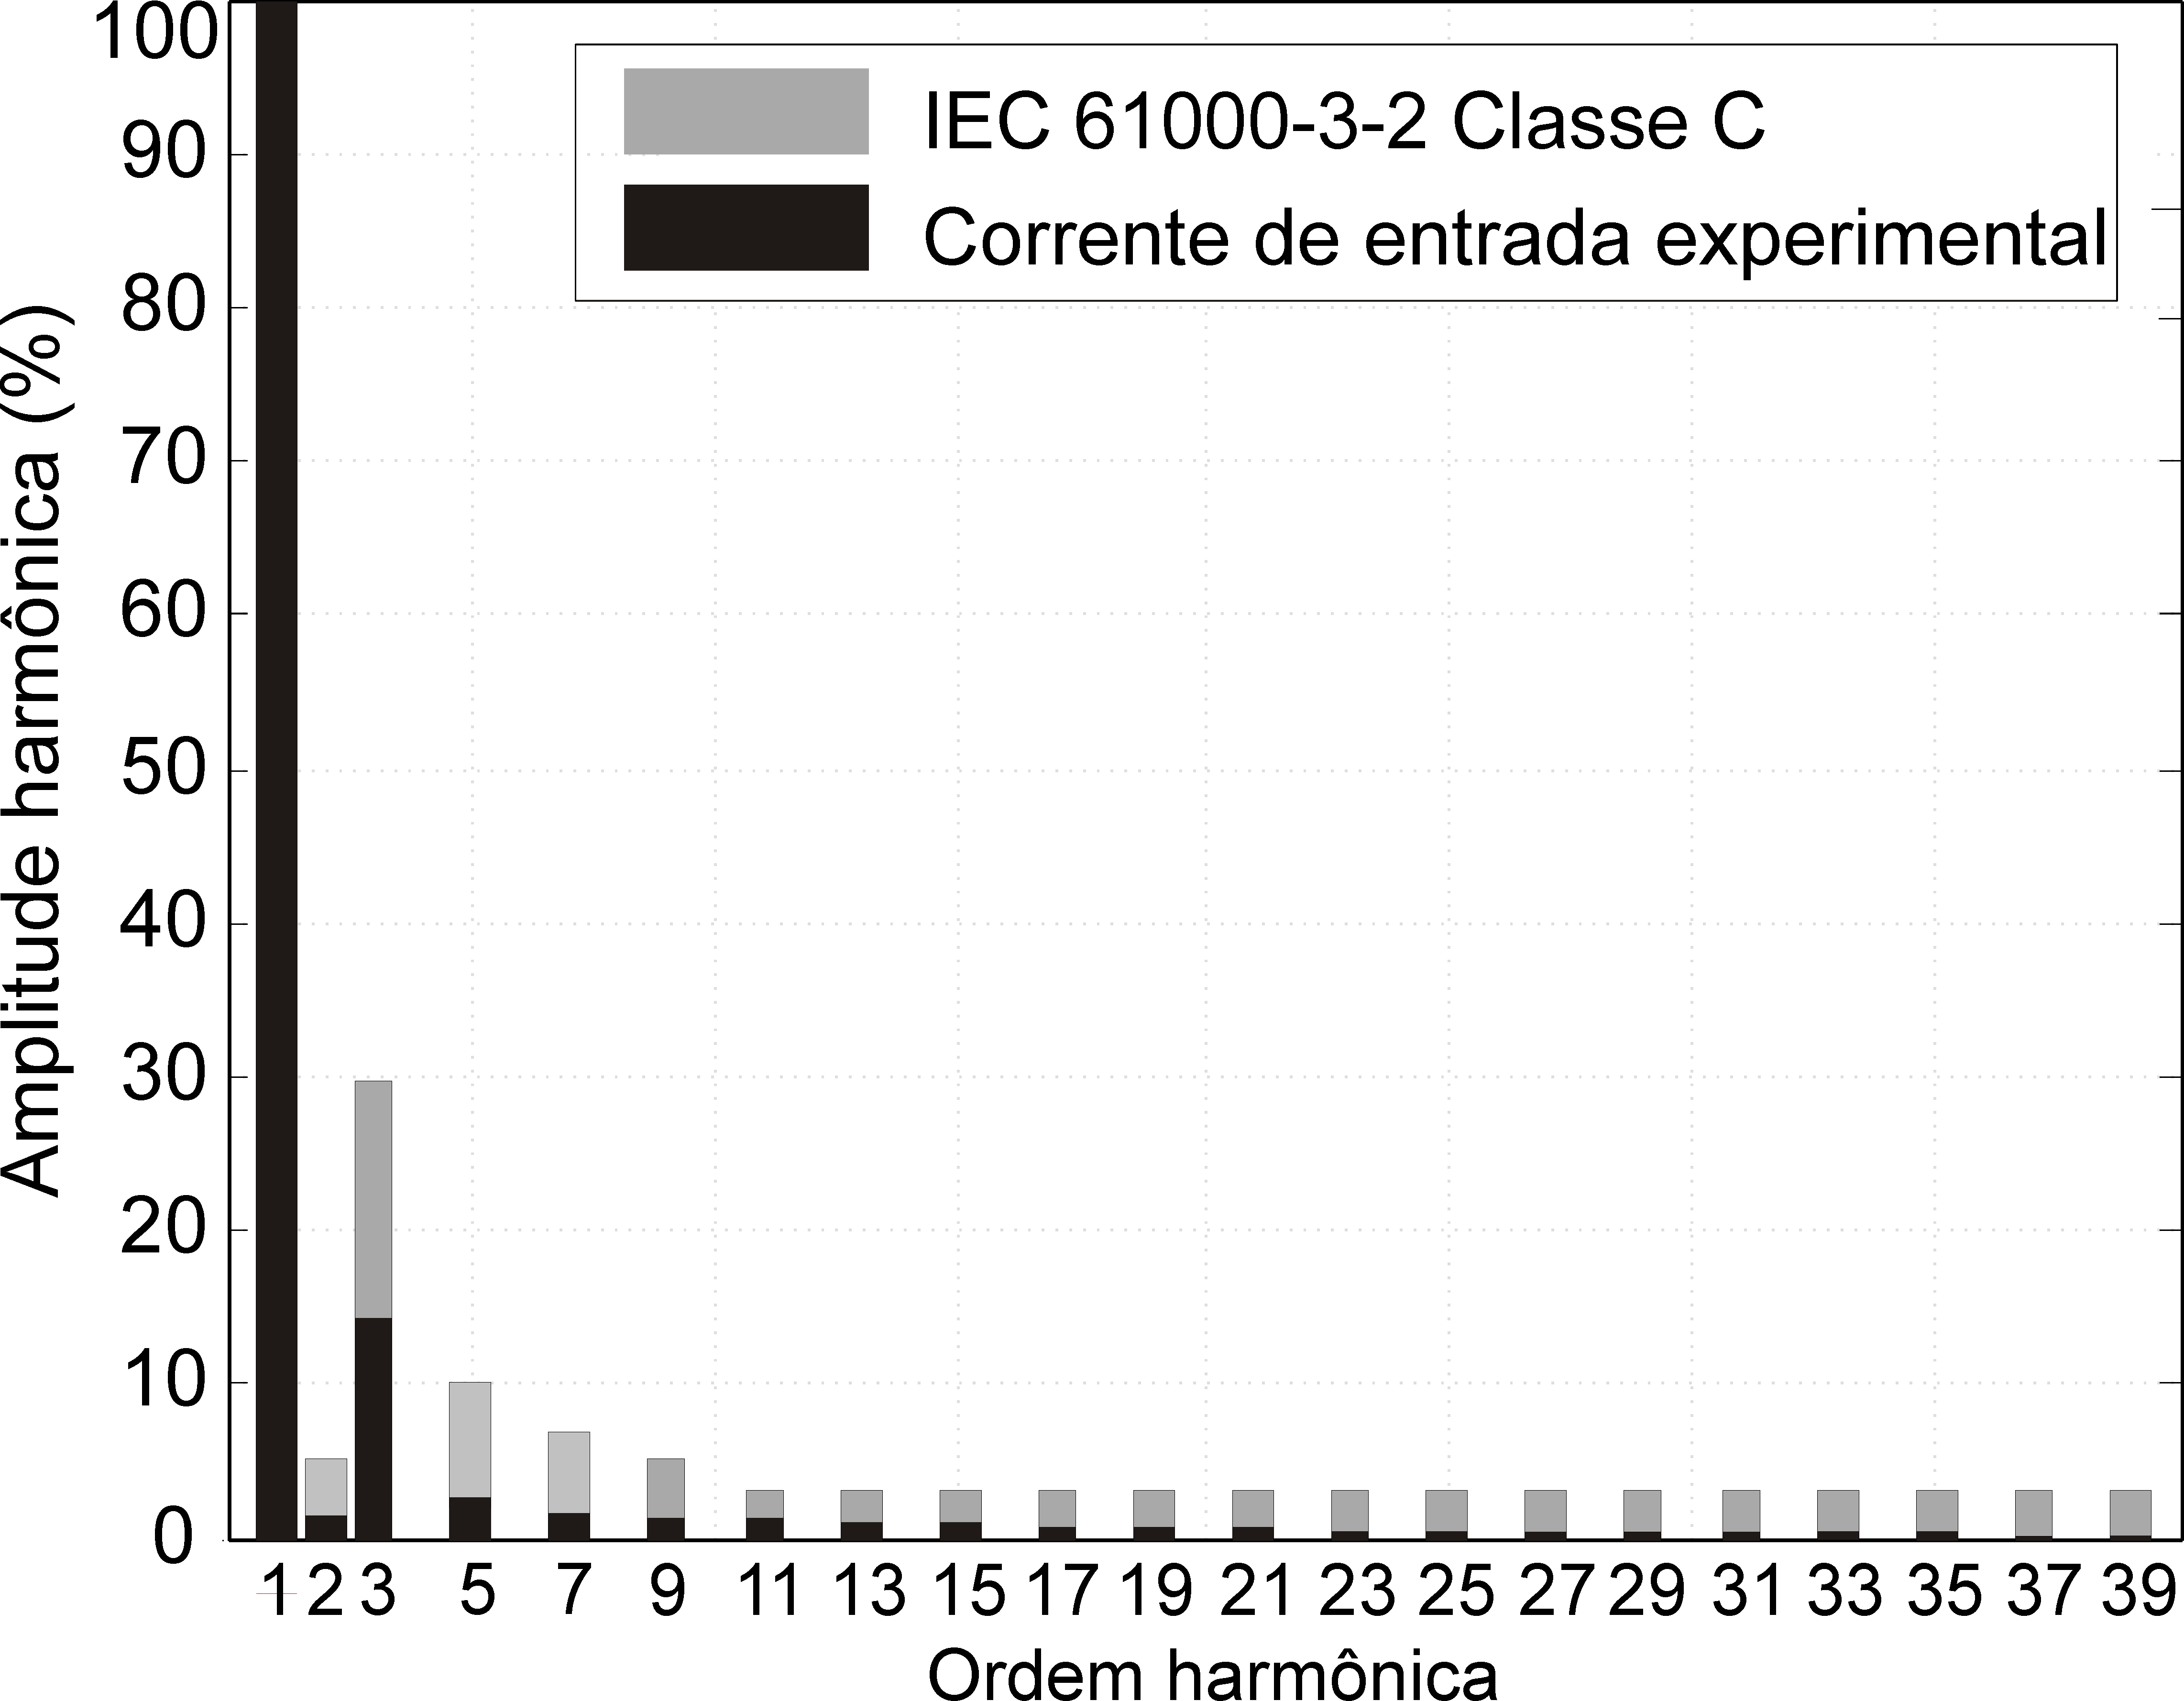
\includegraphics[height=3cm]{../../FIGURAS/Figuras_TFC_Eric/Figuras/iec61000-3-2_controlled_two-stage_pt}}
		}
	\end{figure}
\end{frame}
%----------------------------------------------------------
%----------------------------------------------------------
%----------------------------------------------------------
%----------------------------------------------------------
\begin{frame}{Agradecimentos}
	
		\begin{figure}[htb]
		\centering
		\mbox{
			\subfigure{
				
\includegraphics[height=2cm]{I/NIMO}}\qquad\qquad\qquad
			\subfigure{
				
\includegraphics[height=2cm]{I/UFJF}}
		}
	\end{figure}
	\vspace{5mm}
	\begin{figure}[htb]
		\mbox{
			\subfigure{
				
\includegraphics[height=2cm]{I/capes}}\qquad\qquad\qquad
			\subfigure{
				\includegraphics[height=2cm]{I/LMO}}
		}
	\end{figure}
	
	
\end{frame}
%----------------------------------------------------------

























%\section{Text}
%    \begin{frame}[plain]
%        \vfill
%      \centering
%      \begin{beamercolorbox}[sep=8pt,center,shadow=true,rounded=true]{title}
%        \usebeamerfont{title}\insertsectionhead\par%
%        \color{oxfordblue}\noindent\rule{10cm}{1pt} \\
%        \LARGE{\faFileTextO}
%      \end{beamercolorbox}
%      \vfill
%  \end{frame}


\end{document}

